\documentclass[compress]{beamer}
\mode<presentation>
\usetheme{Warsaw}
\usecolortheme{seagull}
%\useoutertheme[subsection=false]{smoothbars}
\useoutertheme{infolines}
\useinnertheme{rectangles}

\setbeamercovered{dynamic}

\usepackage{array}
\usepackage{amsmath,amssymb,amsfonts,mathrsfs,amsthm}
\usepackage[utf8]{inputenc}
\usepackage{listings}
\usepackage{mathtools}
\usepackage{dsfont}
\usepackage{pdfpages}
\usepackage[textsize=footnotesize,color=green]{todonotes}
\usepackage{algorithm, algorithmic}
\usepackage{bm}
\usepackage{tikz}
\usepackage[normalem]{ulem}

\usepackage{graphicx}
\usepackage{subfigure}
%\usepackage{caption}
%\usepackage{subcaption}

\usepackage{color}
\usepackage{undertilde}
\usepackage{pdflscape}
\usepackage{pifont}

\renewcommand{\topfraction}{0.85}
\renewcommand{\textfraction}{0.1}
\renewcommand{\floatpagefraction}{0.75}

\newcommand{\vect}[1]{\ensuremath\boldsymbol{#1}}
\newcommand{\tensor}[1]{\underline{\vect{#1}}}
\newcommand{\del}{\triangle}
\newcommand{\grad}{\nabla}
\newcommand{\curl}{\grad \times}
\renewcommand{\div}{\grad \cdot}
\newcommand{\ip}[1]{\left\langle #1 \right\rangle}
\newcommand{\eip}[1]{a\left( #1 \right)}
\newcommand{\pd}[2]{\frac{\partial#1}{\partial#2}}
\newcommand{\pdd}[2]{\frac{\partial^2#1}{\partial#2^2}}

\newcommand{\circone}{\ding{192}}
\newcommand{\circtwo}{\ding{193}}
\newcommand{\circthree}{\ding{194}}
\newcommand{\circfour}{\ding{195}}
\newcommand{\circfive}{\ding{196}}

\newcommand{\Reyn}{\rm Re}

\newcommand{\bs}[1]{\boldsymbol{#1}}
\DeclareMathOperator{\diag}{diag}

\newcommand{\equaldef}{\stackrel{\mathrm{def}}{=}}

\newcommand{\tablab}[1]{\label{tab:#1}}
\newcommand{\tabref}[1]{Table~\ref{tab:#1}}

\newcommand{\theolab}[1]{\label{theo:#1}}
\newcommand{\theoref}[1]{\ref{theo:#1}}
\newcommand{\eqnlab}[1]{\label{eq:#1}}
\newcommand{\eqnref}[1]{\eqref{eq:#1}}
\newcommand{\seclab}[1]{\label{sec:#1}}
\newcommand{\secref}[1]{\ref{sec:#1}}
\newcommand{\lemlab}[1]{\label{lem:#1}}
\newcommand{\lemref}[1]{\ref{lem:#1}}

\newcommand{\mb}[1]{\mathbf{#1}}
\newcommand{\mbb}[1]{\mathbb{#1}}
\newcommand{\mc}[1]{\mathcal{#1}}
\newcommand{\nor}[1]{\left\| #1 \right\|}
\newcommand{\snor}[1]{\left| #1 \right|}
\newcommand{\LRp}[1]{\left( #1 \right)}
\newcommand{\LRs}[1]{\left[ #1 \right]}
\newcommand{\LRa}[1]{\left\langle #1 \right\rangle}
\newcommand{\LRc}[1]{\left\{ #1 \right\}}
\newcommand{\tanbui}[2]{\textcolor{blue}{\sout{#1}} \textcolor{red}{#2}}
\newcommand{\Grad} {\ensuremath{\nabla}}
\newcommand{\Div} {\ensuremath{\nabla\cdot}}
\newcommand{\Nel} {\ensuremath{{N^\text{el}}}}
\newcommand{\jump}[1] {\ensuremath{\LRs{\![#1]\!}}}
\newcommand{\uh}{\widehat{u}}
\newcommand{\fnh}{\widehat{f}_n}
\renewcommand{\L}{L^2\LRp{\Omega}}
\newcommand{\pO}{\partial\Omega}
\newcommand{\Gh}{\Gamma_h}
\newcommand{\Gm}{\Gamma_{-}}
\newcommand{\Gp}{\Gamma_{+}}
\newcommand{\Go}{\Gamma_0}
\newcommand{\Oh}{\Omega_h}

\newcommand{\eval}[2][\right]{\relax
  \ifx#1\right\relax \left.\fi#2#1\rvert}

\def\etal{{\it et al.~}}


\def\arr#1#2#3#4{\left[
\begin{array}{cc}
#1 & #2\\
#3 & #4\\
\end{array}
\right]}
\def\vecttwo#1#2{\left[
\begin{array}{c}
#1\\
#2\\
\end{array}
\right]}
\def\vectthree#1#2#3{\left[
\begin{array}{c}
#1\\
#2\\
#3\\
\end{array}
\right]}
\def\vectfour#1#2#3#4{\left[
\begin{array}{c}
#1\\
#2\\
#3\\
#4\\
\end{array}
\right]}

\newcommand{\G} {\Gamma}
\newcommand{\Gin} {\Gamma_{in}}
\newcommand{\Gout} {\Gamma_{out}}

\title{A Discontinuous Petrov-Galerkin method for compressible flow problems}
\author{Jesse Chan \\ Supervisors: Leszek Demkowicz, Robert Moser}

\begin{document}
\begin{frame}
\maketitle
\end{frame}

\section{Introduction/Literature review}
\frame{
\frametitle{Compressible flow problems}
\begin{figure}
\centering
\subfigure[Shock wave]{\includegraphics[scale=.0704]{figs/compFlowPics/bullet_shock.png}}
\subfigure[Boundary layer]{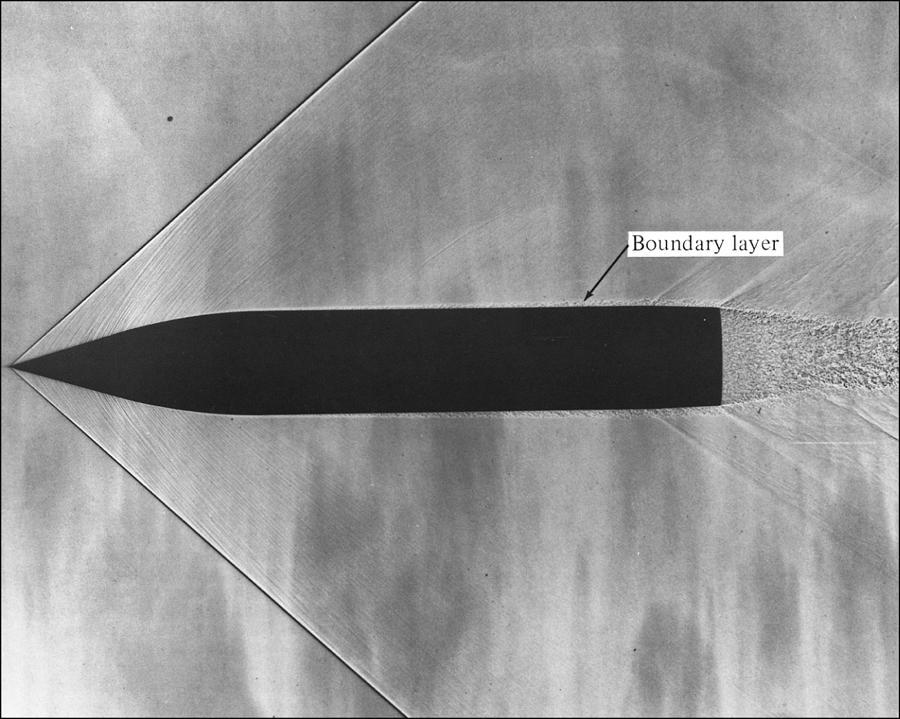
\includegraphics[scale=.16]{figs/compFlowPics/boundary_layer.png}}
%\subfigure{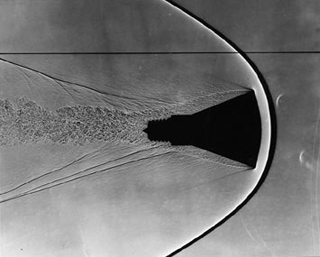
\includegraphics[scale=.15]{figs/compFlowPics/capsule.png}}
\end{figure}
Compressible flow plays an important role in the aerospace and energy industries - transonic and supersonic aircraft, combustion engines, etc. 

}
\frame{
\frametitle{Goal: Compressible Navier-Stokes equations}
\begin{columns}[c]
\begin{column}{.475\textwidth}
Numerical difficulties:
\begin{itemize}
\item{} Resolving solution features (sharp, localized $O(\Reyn^{-1})$ phenomena)
\begin{itemize}
\item{} Shocks, boundary layers
\item{} Turbulent phenomena
\end{itemize}
\item{} Stability of numerical schemes
\begin{itemize}
\item{} Coarse/adaptive grids
\item{} Higher order
\end{itemize}
\item{} Nonlinear convergence and uniqueness of solutions
\end{itemize}
\end{column}
\begin{column}{.475\textwidth}
\begin{figure}
\centering
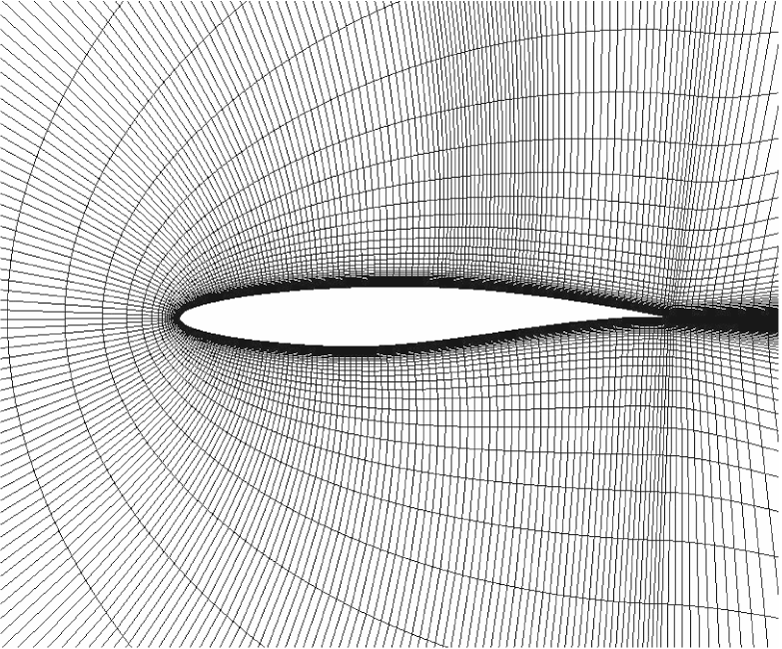
\includegraphics[scale = .7]{figs/compFlowPics/airfoil_mesh.png}
\end{figure}
\end{column}
\end{columns}
\vspace{1cm}
\begin{center}
Idea: begin first with the model problem of convection-diffusion.
\end{center}
}
\frame{
\frametitle{Robustness: convection-diffusion as a model problem}
\vspace{-.5cm}
\[
\div \left(\beta u\right) - \epsilon \Delta u = f, \quad \text{on }\Omega \in \mathbb{R}^3
\]
\vspace{-.5cm}
\begin{columns}[c]
\begin{column}{.49\textwidth}
In 1D: $\beta u' - \epsilon u'' = f$. Standard continuous Galerkin variational formulation: solve
\[
b(u,v) = l(v) 
\]
where
\begin{align*}
b(u,v) &= \int_\Omega -\beta uv' + \epsilon u'v' \\
l(v) &= \int_\Omega f v 
\end{align*}
\end{column}
\begin{column}{.49\textwidth}
\begin{figure}
\centering
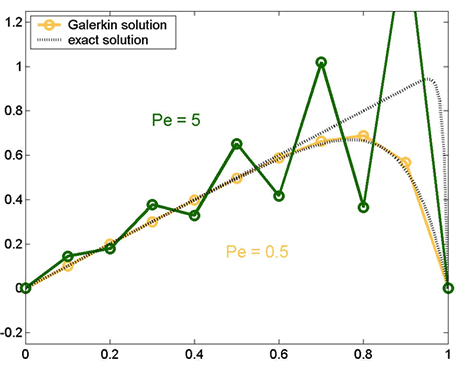
\includegraphics[scale=.35]{figs/GalerkinOscTight.png}
\caption{Oscillations in the standard Galerkin for underresolved meshes and small $\epsilon$.}
\end{figure}
\end{column}
\end{columns}
}
%\frame{
%\frametitle{Stabilization}
%Historical stabilization methods: 
%\begin{itemize}
%\item Artificial diffusion - solve
%\[
%\beta u' - \tilde{\epsilon} u'' = f
%\]
%where $\tilde{\epsilon}$ is set depending on $\beta$, $\epsilon$, and the mesh. Can be made ``exact'' for $f=0$. 
%\item Upwind finite differences - for $\beta > 0$, and uniform grid points $x_A$,
%\[
%u'(x_A) \approx \frac{u_h(x_A)-u_h(x_{A-1})}{h}
%\]
%\end{itemize}
%Both of these methods introduce additional numerical diffusion, and their effectiveness depends on the forcing $f$ and parameters $h$, $|\beta|$, and $\epsilon$.
%}
\frame{
\frametitle{Streamline-upwind Petrov-Galerkin (SUPG)}
SUPG solves $b_{\rm SUPG}(u,v) = l_{\rm SUPG}(v)$, where
\begin{align*}
b_{\rm SUPG}(u,v) &= b(u,v)+ \sum_{K} \int_{K} \tau \LRp{L_{\rm adv} v} L u \\
l_{\rm SUPG}(v) &= l(v) + \sum_{K} \int_{K} \tau \LRp{L_{\rm adv}v} f.
\end{align*}
\vspace{-.5cm}
\begin{columns}[c]
\begin{column}{.47\textwidth}
\vspace{-.5cm}
\begin{itemize}
\item{} $Lu = \div\left(\beta u\right) - \epsilon \triangle u$, $L_{\rm adv}u = \div \left(\beta u\right)$, and $\tau$ is a parameter. 
%\item{} Recovers ``exact'' artificial diffusion for $f=0$.
\item{} Effective for $f\neq 0$, unlike ``exact'' artificial diffusion.
\item{} \emph{Residual-based} stabilization. 
\end{itemize}
\end{column}
\begin{column}{.52\textwidth}
\begin{figure}
\centering
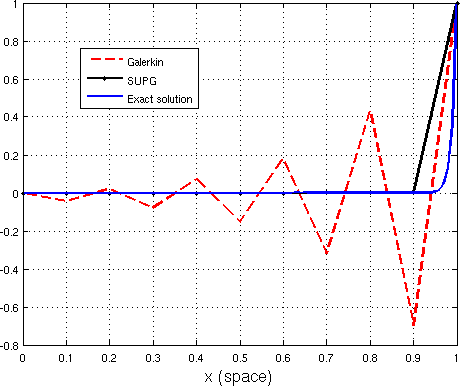
\includegraphics[scale=.35]{figs/SUPG.png}
%\caption{Exact, Bubnov-Galerkin, and SUPG solutions.}
\end{figure}
\end{column}
\end{columns}
}

\frame{
Can be interpreted as a \emph{Petrov-Galerkin} method,
\[
b\LRp{u,\tilde{v}_{i}} = l\LRp{\tilde{v}_{i}}, \quad \forall i = 1,\ldots,N-1,
\]
where the SUPG test function $\tilde{v}_{i}$ is defined elementwise as
\[
\tilde{v}_{i} = \phi_i(x) + \tau L_{\rm adv} \phi_i.  
\]
\begin{figure}
\centering
\subfigure{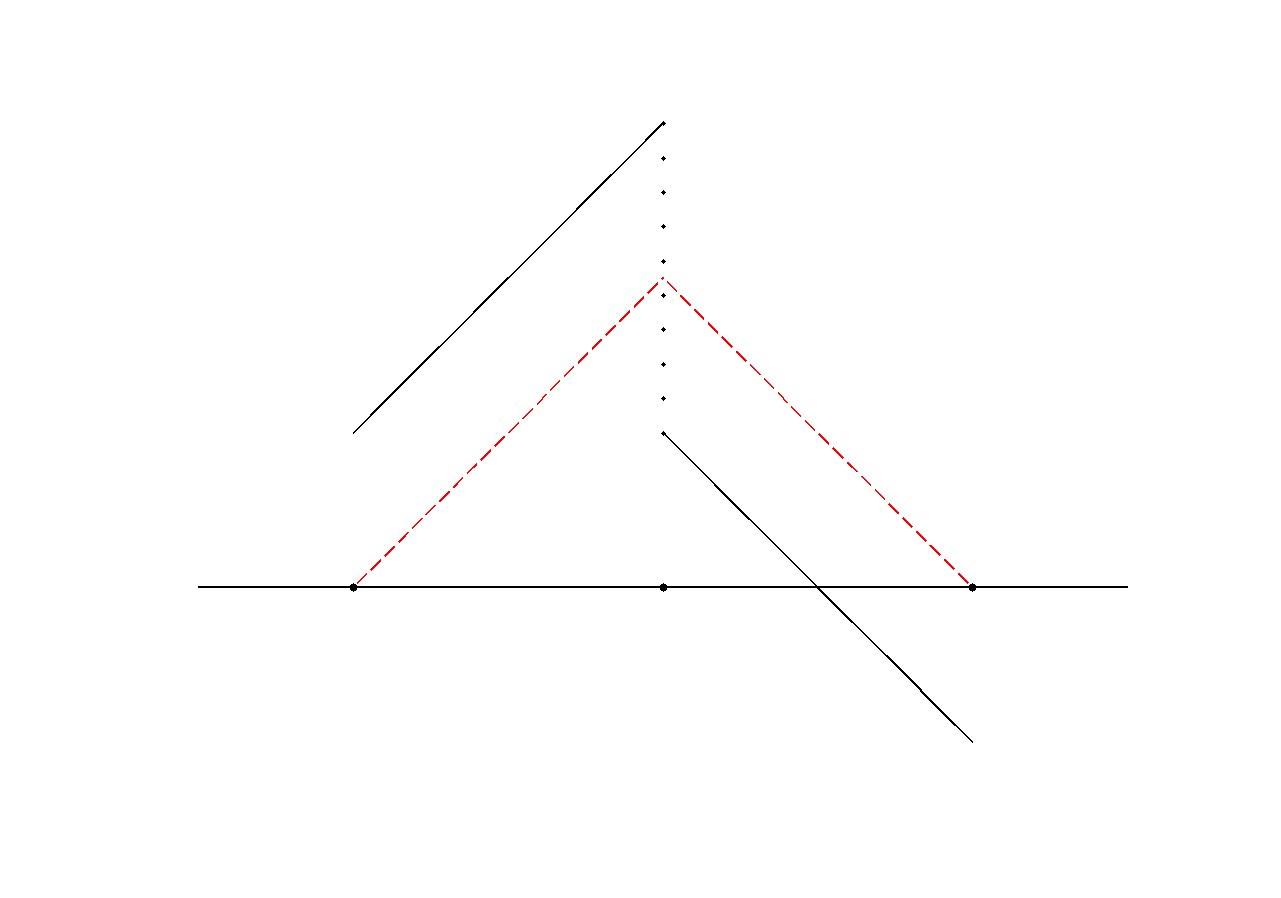
\includegraphics[scale=.185]{figs/SUPGtest.png}}
\caption{SUPG test function $v_i$.}
\end{figure}
}

\section{The DPG Method}
\frame{
\frametitle{DPG: a minimum residual method via optimal testing}
Given
\[
b(u,v) = l(v), \quad u\in U, \quad v\in V
\]
identify $B:U\rightarrow V'$ such that 
\[
\langle Bu,v\rangle_V \coloneqq b(u,v), \quad u\in U, v\in V.
\]
Then, $b(u_h,v) = l(v)$ is equivalent to the equation in $V'$
\[
Bu_h = l
\]
We seek to minimize the functional on $V'$
\[
J(u_h) = \frac{1}{2}\|Bu_h-l\|_{V'}^2 \coloneqq\frac{1}{2} \sup_{v\in V\setminus\{0\}} \frac{| b(u_h,v)-l(v)|^2}{\nor{v}_V^2}.
\]
}

\begin{frame}
Let $R_V: V \to V'$ be the isometric Riesz map st.\
\[
\langle R_V v,\delta v\rangle_V \coloneqq(v, \delta v)_V, \quad \forall \delta v \in V.
\]
Then, our functional $J(u_h)$ is equal to
\begin{equation*}
\min_{u_h\in U_h} J(u_h) = \frac{1}{2}\left\|Bu_h-l\right\|_{V'}^2 =  \frac{1}{2}\left\|R_V^{-1}(Bu_h-l)\right\|_V^2.
\end{equation*}
First order optimality: G\^ateaux derivative is zero in all directions $\delta u \in U_h$
\begin{align*}
\left(R_V^{-1}(Bu_h-l),R_V^{-1}B\delta u\right)_V &= 0, \quad \forall \delta u \in U.\\
\rightarrow \LRa{(Bu_h-l),R_V^{-1}B\delta u} &= 0, \\
\rightarrow b(u_h,R_V^{-1}B\delta u) - l(R_V^{-1}B\delta u) &= 0
\end{align*}
\end{frame}

\frame{
\frametitle{Minimum residual methods and optimal testing}
For $\delta u \in U$, define the \textcolor{red}{optimal test function} $v_{\delta u}$. 
\begin{equation*}
v_{\delta u} \coloneqq R_V^{-1}B\delta u.
\end{equation*} 
Then, the least-squares residual $J(u_h) = \frac{1}{2}\left\|Bu_h-l\right\|_{V'}^2$ is minimized by the solution of
\[
b\LRp{u_h,v_{\delta u}} = l\LRp{v_{\delta u}}, \quad \forall \delta u \in U
\]
}

\frame{
\frametitle{Practical details of DPG}
\begin{itemize}
\item By choosing a \emph{broken} test space $V$ and \textcolor{red}{localizable} norm $\nor{v}_V = \sum_K \nor{v}_{V(K)}$, test functions can be determined locally.
\item In practice, we use the \textcolor{red}{enriched space} $V \coloneqq V_h$, where $\dim(V_h) > \dim(U_h)$ elementwise, and \textcolor{red}{optimal test functions} are approximated by solving
\[
\LRp{v_{\delta u},\delta v}_V = b(\delta u,\delta v), \quad \delta u\in U, \quad v_{\delta u},\delta v\in V_h
\]
Typically, if $U_h = \mathcal{P}^p(\mathbb{R}^n)$, $V_h = \mathcal{P}^{p+\triangle p}(\mathbb{R}^n)$, where $\triangle p \geq n$. 
\end{itemize}
}

\frame{
\frametitle{Properties of DPG}
DPG provides a symmetric positive-definite stiffness matrix. Let $\{\phi_j\}_{j=1}^m$ be a basis for $U_h$, and $\{v_i\}_{i=1}^n$ a basis for $V_h$, such that $n>m$. Then, for 
\begin{align*}
B_{ji} &= b(\phi_j,v_i),\\
l_i &= l(v_i),
\end{align*}
DPG solves the discrete system
\begin{align*}
(B^T R_V^{-1}B) u  &= (B^T R_V^{-1}) l,
\end{align*}
where, under a localizable norm and discontinuous test functions, $R_V^{-1}$ is block diagonal.
}

\frame{
\frametitle{Properties of DPG}
\begin{itemize}
\item DPG provides the best approximation in the \textcolor{red}{energy norm}
\[
\|u\|_E = \|Bu\|_{V'} = \sup_{\nor{v}_V=1} \left|b(u,v)\right|.
\]
\item The energy error is computable through the residual
\[
\nor{u-u_h}_E = \nor{B(u-u_h)}_{V'} = \nor{R_V^{-1}(l-Bu_h)}_V = \nor{e}_V
\]
where the \textcolor{red}{error representation function} $e$ is defined through $(e,\delta v)_V = l(v)-b(u_h,\delta v)$ for all $\delta v\in V$. 
\end{itemize}
}

%\frame{
%\frametitle{Duality of norms}
%Duality of norms: for any trial norm $\nor{u}_U$,
%\[
%\nor{u}_{U} = \sup_{v \in V}\frac{b\LRp{u,v}}{\nor{v}_{V,U}}, \quad \nor{v}_{V,U} = \sup_{u \in U}\frac%{b\LRp{u,v}}{\nor{u}_{U}}.
%\]
%Likewise, for any test norm $\nor{v}_V$, 
%\[
%\nor{v}_{V} = \sup_{u \in U}\frac{b\LRp{u,v}}{\nor{U}_{U,V}}, \quad \nor{u}_{U,V} = \sup_{v \in V}\frac%{b\LRp{u,v}}{\nor{v}_{V}}.
%\]
%
%}

\frame{
\frametitle{Ultra-weak formulation}
\vspace{-.75cm}
\begin{columns}
\begin{column}{.65\textwidth}
Given a first order system $Au = f$, we identify the \textbf{\emph{partition}} $\Oh$ and \textbf{\textcolor{red}{mesh skeleton}} \textcolor{red}{$\Gh$}.
\end{column}
\begin{column}{.33\textwidth}
%\[
%\Oh = \cup_{j=1}^\Nel K_j, \quad \Gh = \cup_{j=1}^\Nel \partial K_j
%\]
\begin{figure}[!h]
\centering
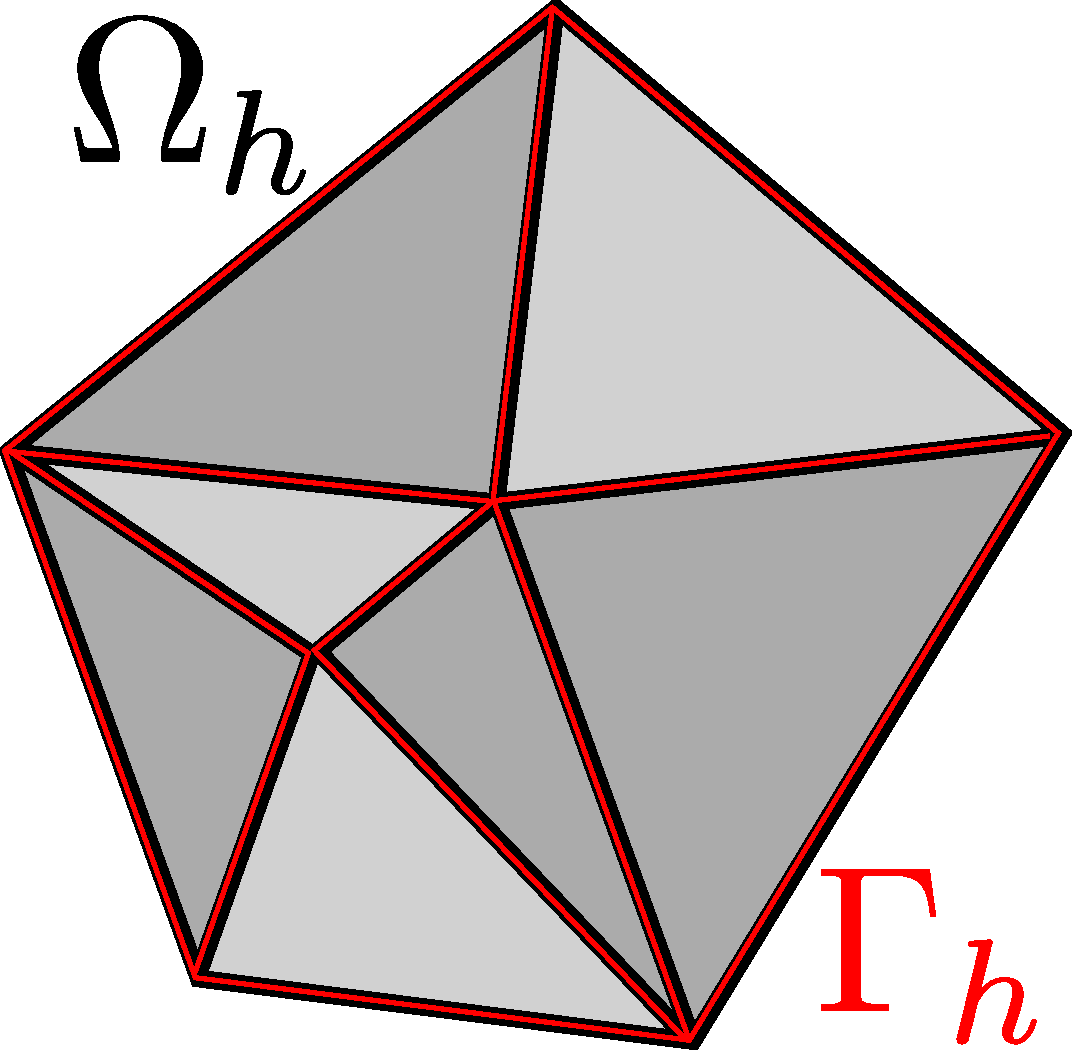
\includegraphics[scale = .155]{mesh_skel.pdf}
\end{figure}
\end{column}
\end{columns}
\vspace{-.5cm}
The ultra-weak formulation for $Au = f$ on $\Oh$ is
\[
b\left(\left(u, \widehat{u}\right),v\right) \coloneqq \sum_K\langle \widehat{u},v \rangle_{\delta K} + (u,A_h^*v)_{\Oh}= \LRp{f,v}_{\Oh}.
\]
Under proper assumptions, $\sum_K\langle \widehat{u},v \rangle_{\delta K} = \langle \widehat{u}, \jump{v} \rangle_{\Gh}$. The energy setting is
\[
u\in L^2\LRp{\Oh} \equiv L^2(\Omega), \quad v\in V=D(A^*_h), \quad
\widehat{u}\in \gamma(D(A)),
\]
where $D(A_h^*)$ is the broken graph space of the formal adjoint $A_h^*$, and $\gamma(D(A))$ the trace space of the graph space of operator $A$.
}

\frame{
\frametitle{Test and trial norms for the ultra-weak formulation}
Under the ultra-weak formulation, we have the following equivalence relations:
\begin{figure}[!h]
\centering
\begin{tabular}{l c c}
Trial norm & & Test norm \\
\hline
$\boxed{\|u\|^2_{\L} + \|\widehat{u}\|^2}$ & $\Longrightarrow$  & $\|A_h^*v\|_{\L}^2
+\left(\sup_{\widehat{u}} \frac{\LRa{ \widehat{u},
  \jump{v} }_{\Gh}}{\|\widehat{u}\|}\right)^2$ \\
$\nor{u}_{\L}^2+\sup_{v } \left(\frac{\LRa{\widehat{u},
  \jump{v}}_{\Gh}}{\|v\|_V}\right)^2$ &  $\Longleftarrow$ & $\boxed{\|A_h^*v\|_{\L}^2 + \nor{v}_{\L}^2}$
\end{tabular}
\caption{The optimal \textit{test} norm is naturally derived by beginning with the canonical norm on the trial space, while the quasi-optimal \textit{trial} norm is derived from beginning with the canonical (\emph{graph}) norm on the test space.}
\end{figure}
}

%\frame{
%\frametitle{The canonical test norm}
%Under the ultra-weak formulation, we have the natural norm
%\[
%\nor{\LRp{u,\widehat{u}}} = \|u\|^2_{\L} + \|\widehat{u}\|^2 
%\]
%which generates a test norm \emph{equivalent} to 
%\[
%\nor{v}_{V_{\rm opt}} \coloneqq \|A_h^*v\|_{\L}^2 +\left(\sup_{\widehat{u}} \frac{\LRa{ \widehat{u},\jump{v} }_{\Gh}}{\|\widehat{u}\|}\right)^2
%\]
%This norm is not localizable, so we instead substitute the jump terms for an $L^2$ term, giving us the \emph{graph norm}
%\[
%\nor{v}_V \coloneqq \|A_h^*v\|_{\L}^2 + \nor{v}_{L^2}.
%\]
%}

\section{A Robust DPG Method for Convection-Diffusion}

\frame{
\frametitle{Ultra-weak formulation for convection-diffusion}
In first order form, the convection-diffusion equation is
\[
A \LRp{u,\sigma} \coloneqq 
\LRs {
\begin{array}{c}
\div (\beta u - \sigma) \\ \frac{1}{\epsilon}\sigma - \grad u
\end{array}} = \LRs{
\begin{array}{c}
f \\ 0
\end{array}
}.
\]
The variational formulation is
\begin{align*}
b\left(\left(u,\sigma, \widehat{u}, \widehat{f}_n\right),
\left( v, \tau \right)\right) = \left(u,\grad_h\cdot \tau - \beta \cdot \grad_h
v\right)_{\Oh} + \left(\sigma, \epsilon^{-1} \tau + \grad_h v\right)_{\Oh}&\\
 - \LRa{\jump{\tau\cdot n}, \widehat{u} }_{\Gh} + \LRa{ \widehat{f}_n,\jump{v} }_{\Gh}&,
\end{align*}
where $\widehat{f}_n \coloneqq \beta_n u - \sigma_n$, and $\grad_h\cdot$ and $\grad_h$ act elementwise.
}

\frame{
\frametitle{Graph norm under convection-diffusion}
For convection-diffusion, the quasi-optimal (graph) test norm is 
\[
\|\left(v,\tau\right)\|_V^2 = \| \div \tau - \beta \cdot \grad v
\|_{L^2}^2 + \| \epsilon^{-1} \tau + \grad v \|_{L^2}^2 +
\|v\|_{L^2}^2.
\]
Problem with this test norm: approximability of test functions.
\vspace{-.3cm}
\begin{figure}[!h]
\centering
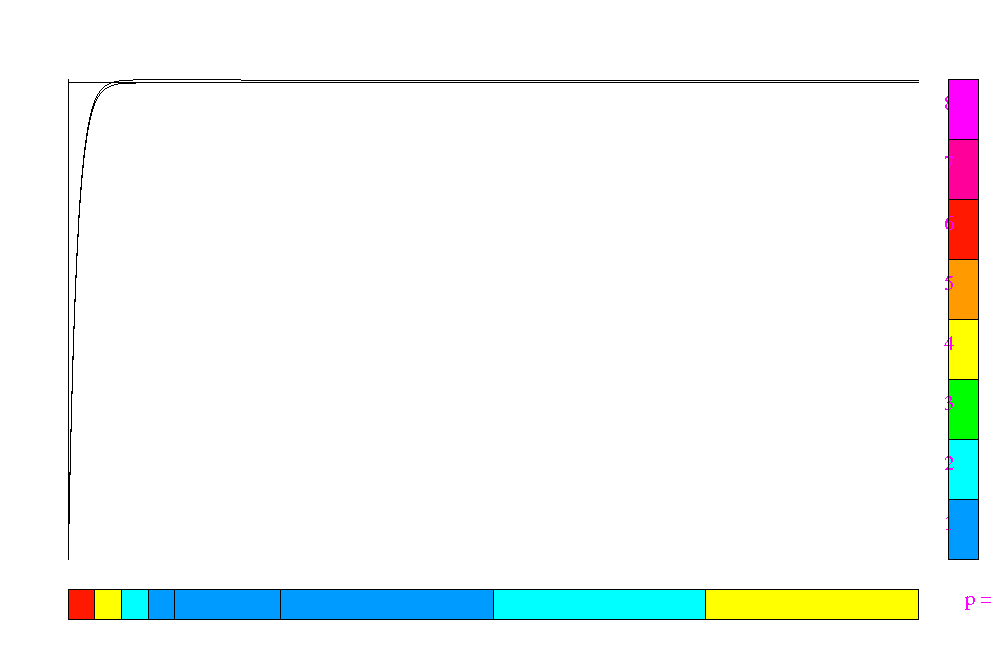
\includegraphics[scale=.175]{figs/opt.png}
\caption{$v$ and $\tau$ components of the 1D optimal test functions for flux $\widehat{f}_n$ on the \emph{right-hand} side of a unit element for $\epsilon = 0.01$. }
\label{fig:optTestBoundary}
\end{figure}
}

\frame{
\frametitle{Determining an alternative test norm}
Recall the convection-diffusion bilinear form
\begin{align*}
b\left(\left(u,\sigma, \widehat{u}, \widehat{f}_n\right),
\left( v, \tau \right)\right) = \left(u,\div \tau - \beta \cdot \grad
v\right)_{\Oh} + \left(\sigma, \epsilon^{-1} \tau + \grad v\right)_{\Oh}&\\
 - \LRa{\jump{\tau\cdot n}, \widehat{u} }_{\Gh} + \LRa{ \widehat{f}_n,\jump{v} }_{\Gh}&,
\end{align*}
We recover $\nor{u}_{L^2(\Omega)}$ by choosing continuous $\LRp{v,\tau}$ satisfying the \emph{adjoint equations}
\begin{align*}
\div\tau - \beta \cdot \grad v   &= u\\
\frac{1}{\epsilon}\tau + \grad v &= 0
\end{align*}
where boundary conditions are s.t.\ $\LRa{\jump{\tau\cdot n}, \widehat{u} }_{\Gh}$ and $\LRa{ \widehat{f}_n,\jump{v} }_{\Gh}$ vanish. 
}

\frame{
\frametitle{A robust bound}
``Necessary'' conditions for robustness --- let $\boldsymbol U = \LRp{u,\sigma,\widehat{u},\widehat{f}_n}$, then, by choosing specific $\LRp{v,\tau}$ satisfying the adjoint equations,
\[
\nor{u}^2_{L^2(\Omega)} = b\LRp{{\boldsymbol U},\LRp{v,\tau}} = \frac{b\LRp{{\boldsymbol U},\LRp{v,\tau}}}{\nor{\LRp{v,\tau}}_V} \nor{\LRp{v,\tau}}_V \leq \nor{\boldsymbol U}_E \nor{\LRp{v,\tau}}_V
\]
If $ \nor{\LRp{v,\tau}}_V \lesssim \|u\|_{L^2(\Omega)}$, then we have the robust bound
\[
\nor{u}_{L^2(\Omega)} \lesssim \nor{\boldsymbol U}_E
\]
\textbf{Test norm should measure the adjoint solution robustly.}
}
\frame{
\frametitle{Dirichlet inflow boundary condition}
Standard choice of boundary condition: $u = u_0$ on inflow boundary $\Gamma_{\rm in}$, induces boundary layers in adjoint problems. 
\begin{figure}[h!]
\centering
\subfigure[Primal problem]{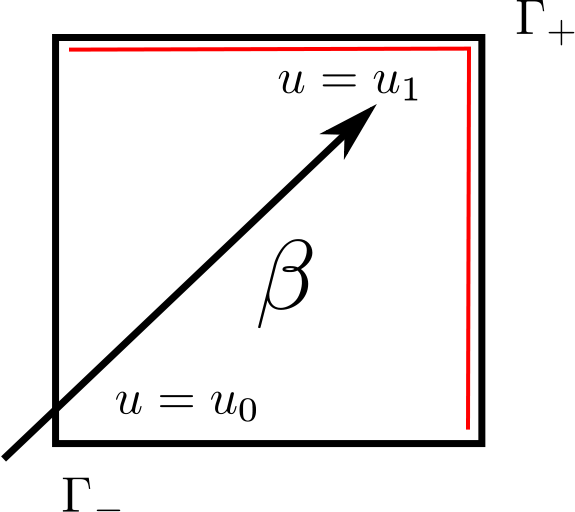
\includegraphics[scale=.23]{figs/primalDir.png}}
\subfigure[Adjoint problem]{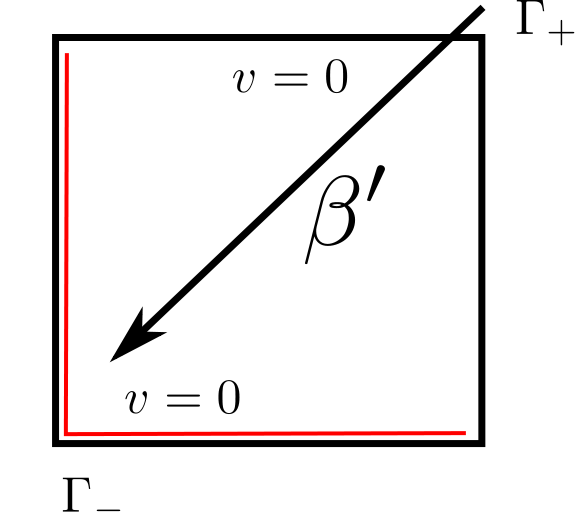
\includegraphics[scale=.23]{figs/adjointDir.png}}
\caption{For the standard Dirichlet inflow condition, the solution to the adjoint problem can develop strong boundary layers at the outflow of the adjoint problem. }
\end{figure}
}

\frame{
\frametitle{New inflow boundary condition on $\widehat{f}_n$}
Non-standard choice of boundary condition: $\widehat{f}_n = \beta_n u_0$ on $\Gamma_{\rm in}$, induces smoother adjoint problems. 
\begin{figure}[h!]
\centering
\subfigure[Primal problem]{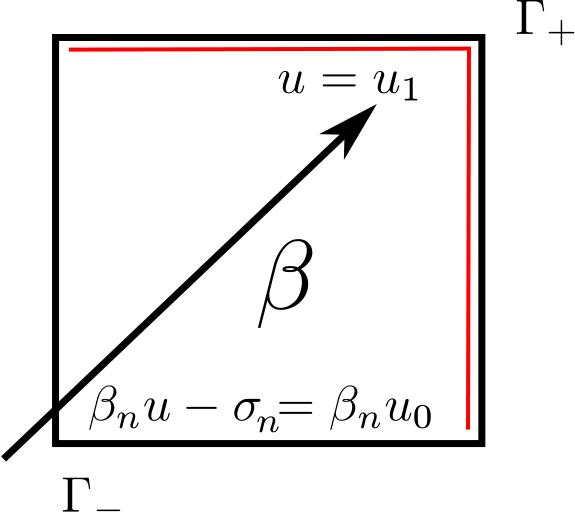
\includegraphics[scale=.23]{figs/primal.png}}
\subfigure[Adjoint problem]{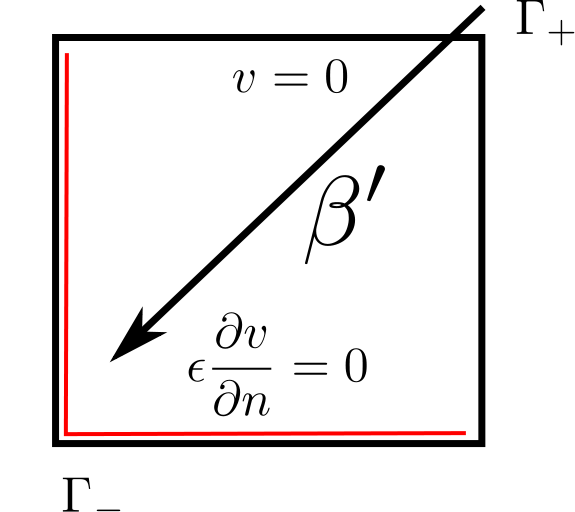
\includegraphics[scale=.23]{figs/adjoint.png}}
\caption{Under the new inflow condition, the wall-stop boundary condition is relaxed to a zero-stress condition at the outflow boundary of the adjoint problem.}
\end{figure}
}

\frame{
\frametitle{Test norms and adjoint solutions}
\textbf{Intuition:} the effectiveness of DPG under a test norm is governed by how a \textbf{specific test norm} measures the \textbf{solutions of the adjoint problem}. 

\begin{figure}[!h]
\subfigure[Dirichlet inflow]{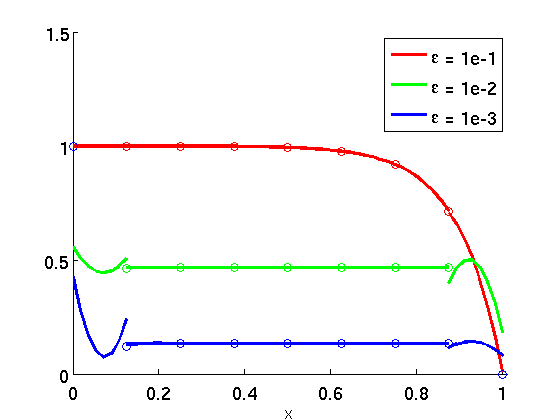
\includegraphics[scale=.35]{figs/dirichletBC.png}}
\subfigure[``Convection'' inflow]{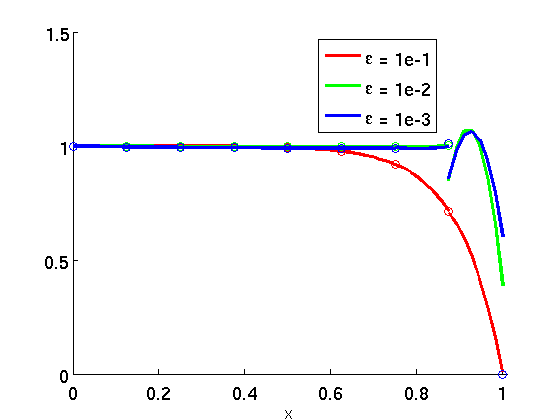
\includegraphics[scale=.35]{figs/newBC.png}}
\caption{DPG solutions to convection-diffusion for both inflow conditions using an $H^1$ test norm.}
\end{figure}
}

%\frame{
%\frametitle{``Building blocks'' norm}
%Test norm quantities are robustly bounded from above by $\nor{u}_{L^2(\Omega)}$.  
%\[
%\|\left(v,\tau\right)\|_{V,K}^2 = \|v\|^2 + \epsilon \|\grad v\|^2 + \|\beta \cdot \grad v\|^2 + \| \div \tau\|^2 + \frac{1}{\epsilon}\|\tau\|^2.
%\]
%Problem: boundary layers in optimal test functions:
%\begin{figure}[!h]
%\centering
%\subfigure{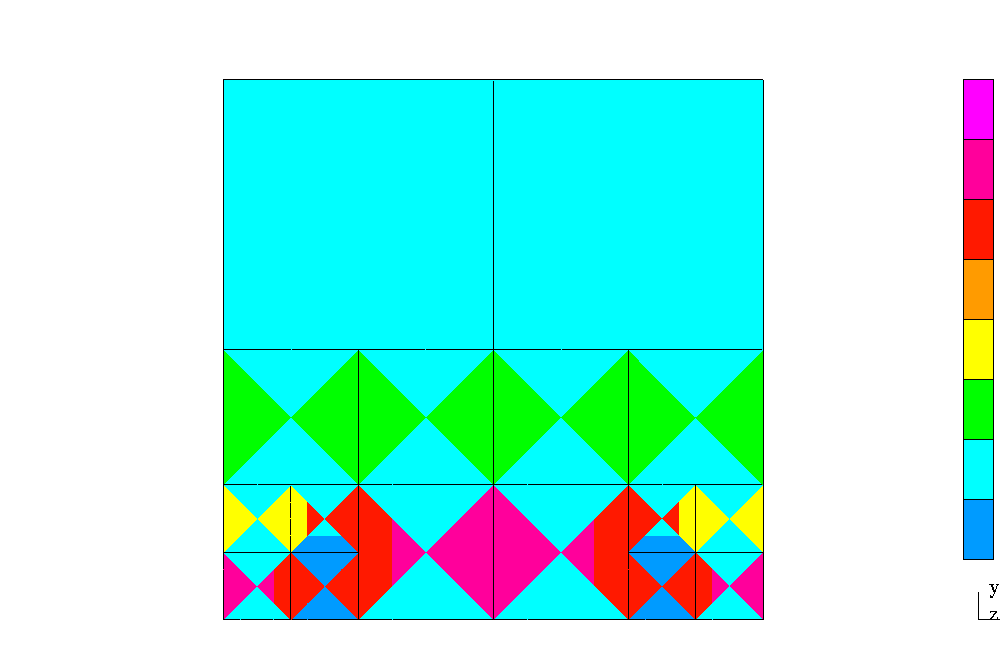
\includegraphics[scale=.15]{figs/mesh1.png}}
%\subfigure{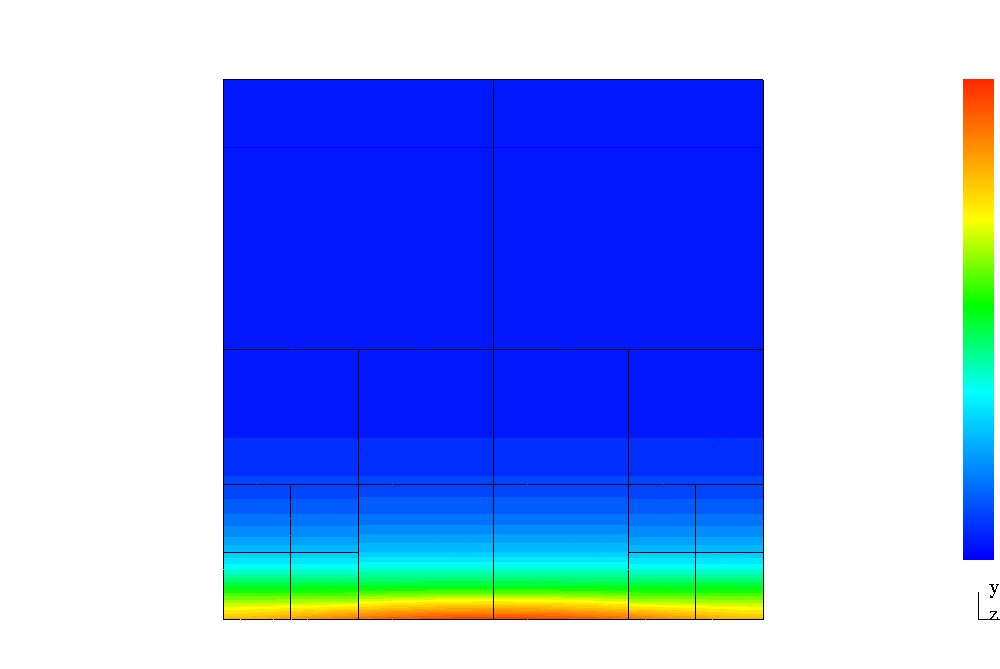
\includegraphics[scale=.15]{figs/sol1.png}}
%\caption{The $v$ component of the optimal test function corresponding to flux $\widehat{u} = x(1-x)$ on the bottom side of a unit element for $\epsilon = 0.01$.}
%\label{fig:boundaryTest}
%\end{figure}
%}
\frame{
\frametitle{Adjoint estimates, or ``norm building blocks''}
For solutions $(v,\tau)$ of the adjoint equations, the following quantities are robustly bounded from above by $\nor{u}_{L^2(\Omega)}$.  
\begin{align*}
&\|v\|, \sqrt{\epsilon} \|\grad v\|, \|\beta \cdot \grad v\| \\
&\| \div \tau\|, \frac{1}{\sqrt{\epsilon}}\|\tau\|.
\end{align*}
We will construct a test norm through a combination of the above quantities, such that
\begin{itemize}
\item $v$ and $\tau$ decoupled (no systems).
\item Coefficients are of equal order after transforming to the unit element (no boundary layers).
\end{itemize}
}
\frame{
\frametitle{Mesh-scaled test norms}
Our test norm, as defined over a single element $K$, is now
\begin{align*}
\|\left(v,\tau\right)\|_{V,K}^2 = \min\left\{\frac{\epsilon}{|K|},1\right\}\|v\|^2 + \epsilon \|\grad v\|^2 + \|\beta \cdot \grad v\|^2 +&\\
\| \div \tau\|^2 + \min\left\{\frac{1}{\epsilon},\frac{1}{|K|}\right\}\|\tau\|^2&.
\end{align*}
which induces the proven \emph{robust} bound 
\[
\nor{u}_{L^2(\Omega)}+ \nor{\sigma}_{L^2(\Omega)} + \epsilon\nor{\widehat{u}} + \sqrt{\epsilon} \nor{\widehat{f}_n} \lesssim \nor{\LRp{u,\sigma,\widehat{u},\widehat{f}_n}}_E.
\]
}


\frame{
\frametitle{Erikkson-Johnson model problem}

On domain $\Omega = [0,1]^2$, with $\beta = (1,0)^T$, $ f = 0$ and boundary conditions
\begin{align*}
\widehat{\beta_nu - \sigma_n} &= \widehat{f_n} = u_0, \quad \beta_n \leq 0\\
\widehat{u} &= 0, \quad \beta_n > 0
\end{align*}

Separation of variables gives an analytic solution. 
%\[
%u(x,y) = C_0 + \sum_{n=1}^\infty C_n \frac{\exp(r_2(x-1)-\exp(r_1(x-1)))}{r_1\exp(-r2) - r_2\exp(-r1)}\cos(n\pi y)
%\]
\begin{figure}
\centering
\subfigure{
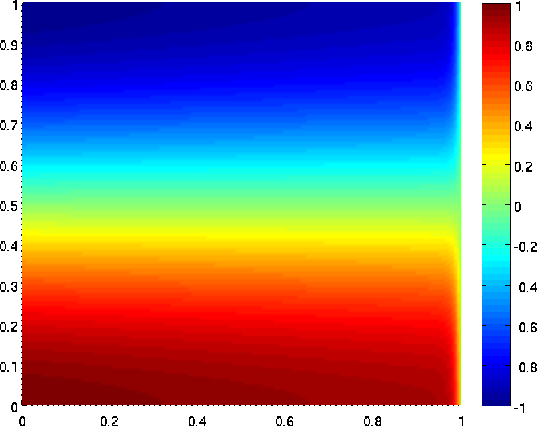
\includegraphics[scale=.24]{figs/wallBC_exact_u.png}
}
\subfigure{
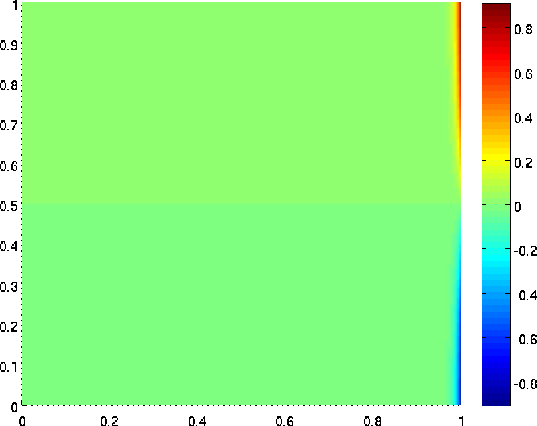
\includegraphics[scale=.24]{figs/wallBC_exact_sigx.png}
}
\subfigure{
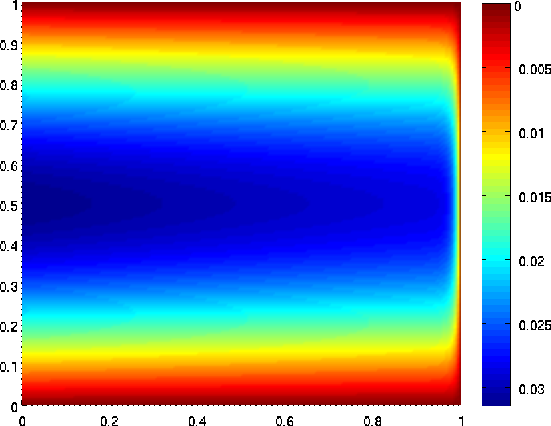
\includegraphics[scale=.24]{figs/wallBC_exact_sigy.png}
}
\caption{Solution for $u$, $\sigma_x$, and $\sigma_y$ for $\epsilon = .01$, $C_1 = 1$, $C_n=0$, $n\neq 1$}
\end{figure}

}

\frame{
\frametitle{Error rates}
\begin{figure}
\centering
\subfigure{
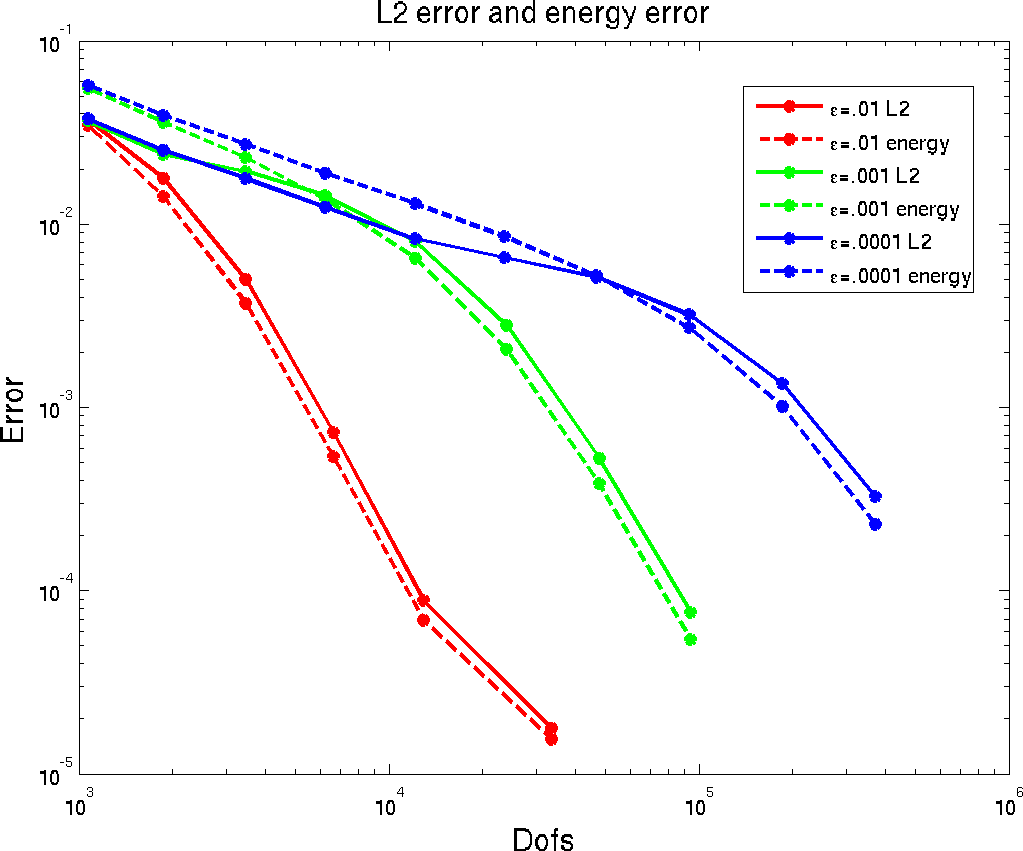
\includegraphics[scale=.24]{figs/errorrates_wallBC.png}
}
\subfigure{
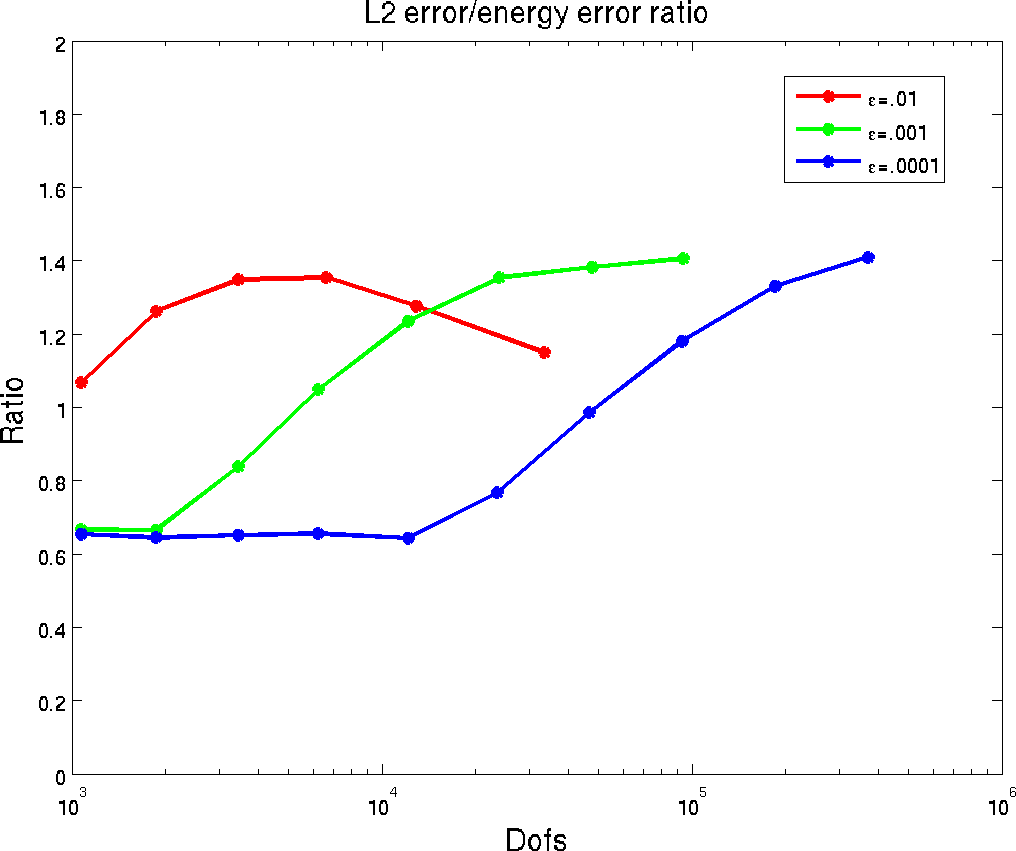
\includegraphics[scale=.24]{figs/L2energyratio_wallBC.png}
}
\subfigure{
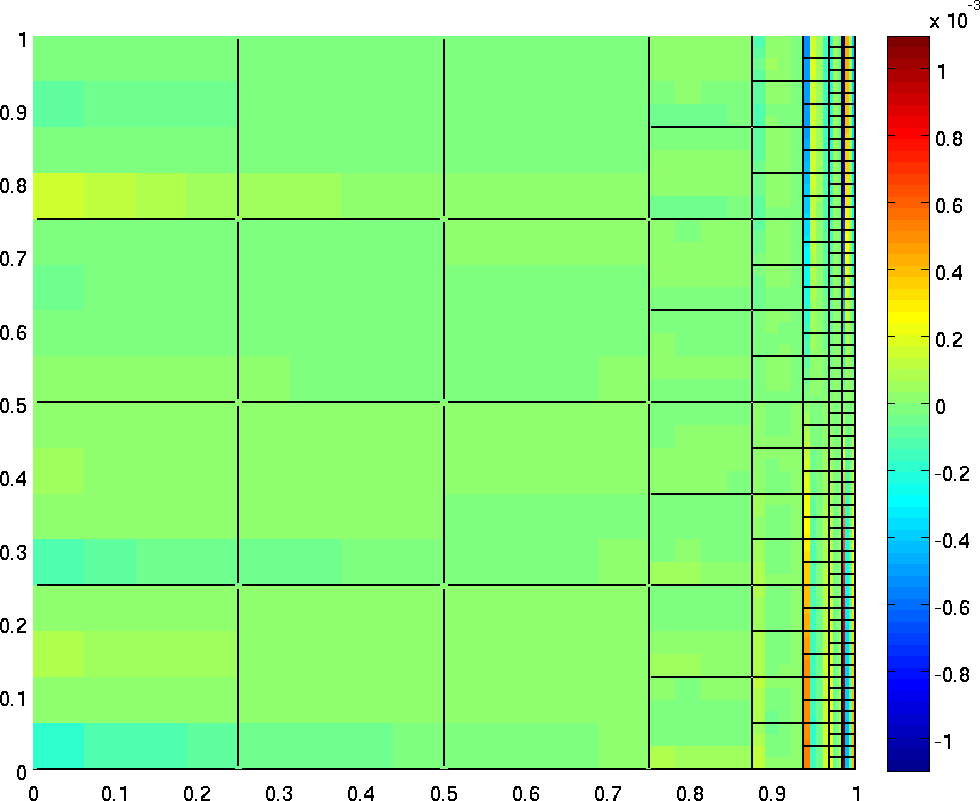
\includegraphics[scale=.22]{figs/u_pointdiff_wallBC.png}
}
\caption{$L^2$/energy error, their ratio, and pointwise error in $u$ for $\epsilon = .01$.}
\end{figure}
}

%\frame{
%\frametitle{Regularization}
%Discontinuous inflow conditions on $\widehat{f_n}$, out of alignment with mesh. Boundary condition $\epsilon \grad u \cdot n = 0$ at outflow.
%\begin{figure}
%\centering
%\subfigure{
%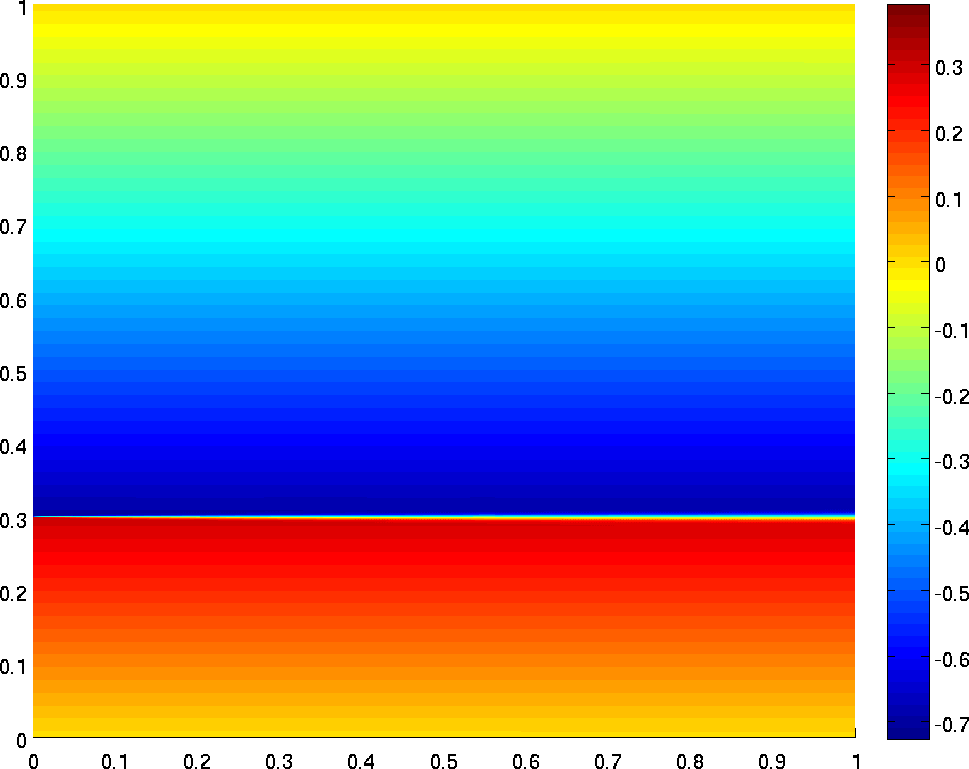
\includegraphics[scale=.33]{figs/discontinuous.png}
%}
%\subfigure{
%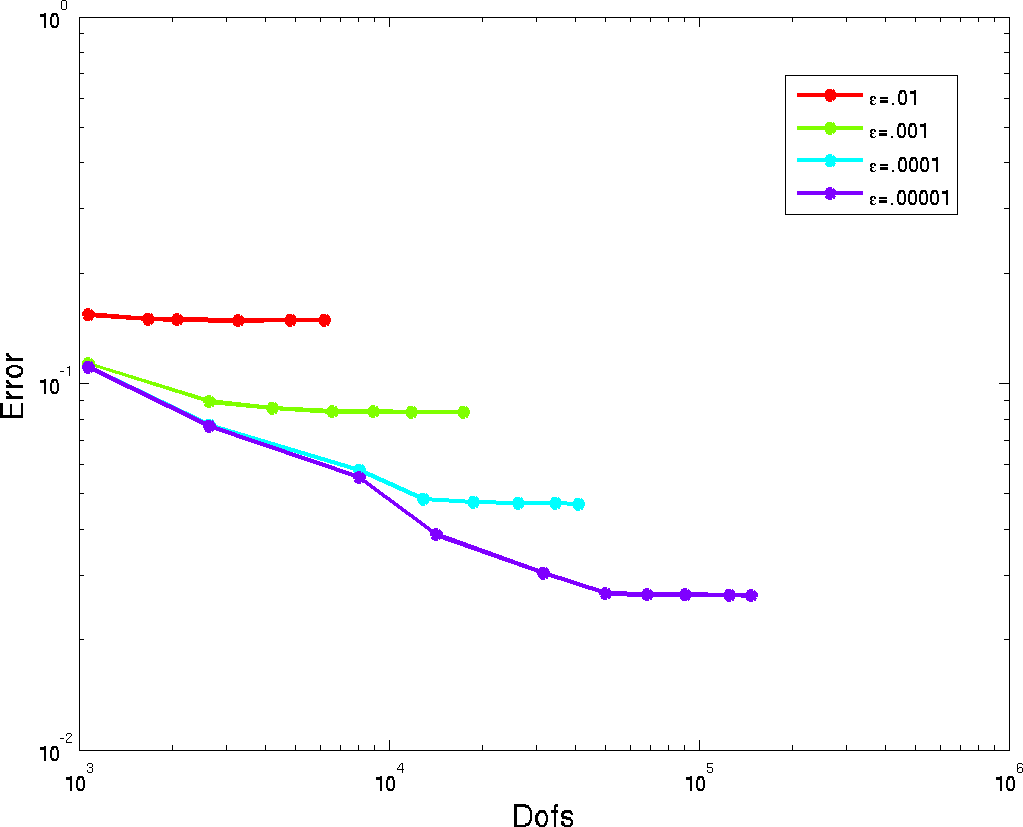
\includegraphics[scale=.305]{figs/discontinuousL2rates.png}
%}
%\caption{Discontinuous hat inflow data with $\epsilon = 1e-5$, convection solution errors.}
%\end{figure}
%}

\frame{
\frametitle{Regularization}
For $\beta = (.5-y,x-.5)^T$ on $\Omega = [0,1]^2$, and zero normal stress outflow conditions. Ill posed in the convection setting. Similar tests have been done with discontinuous data.

\begin{figure}
\centering
\subfigure{

\includegraphics[scale=.35]{figs/vortex.png}
}
\subfigure{
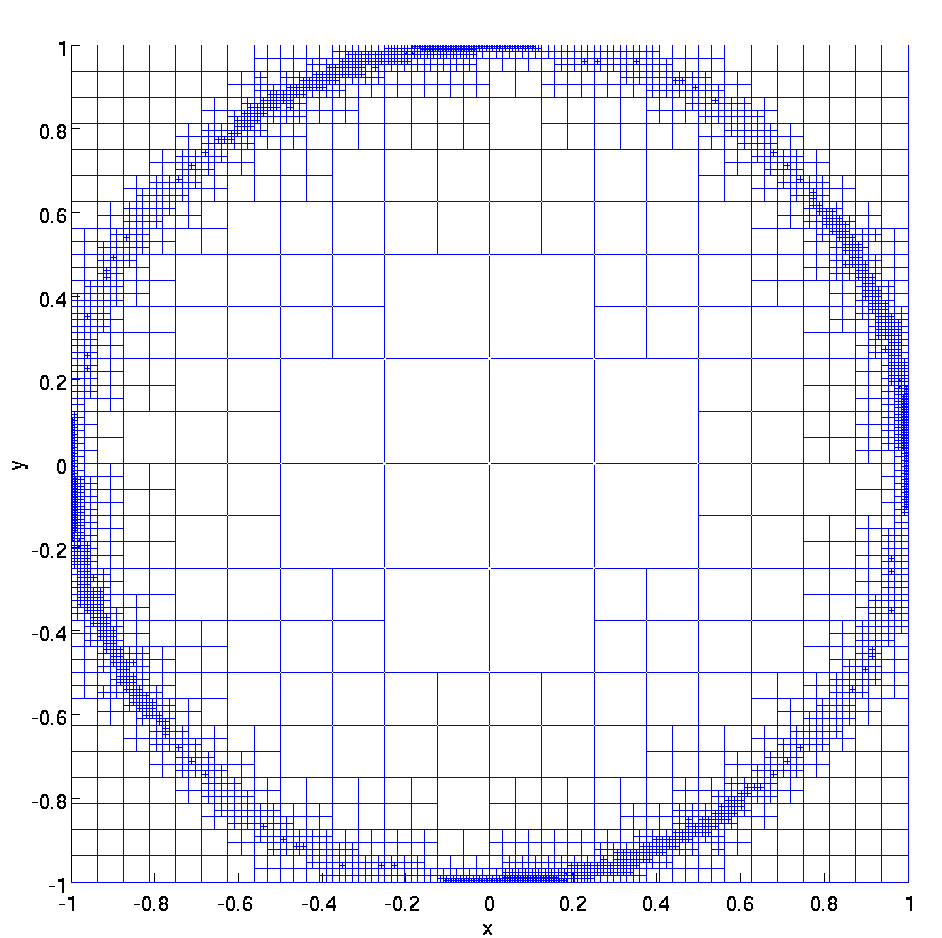
\includegraphics[scale=.35]{figs/vortexMesh.png}
}
\caption{Steady-state vortex problem with $\epsilon = 1e-5$.}
\end{figure}
\vspace{-.25cm}
}

\section{DPG for nonlinear problems}
\frame{
\frametitle{DPG for nonlinear problems}

Given some linearization technique, we can measure 
\begin{itemize}
\item size of the linearized update $\Delta u$
\[
\|\Delta u\|_E \coloneqq \nor{B_u\Delta u}_{V'} = \nor{R_V^{-1} B_u\Delta u}_V 
\]
\item the nonlinear residual 
\[
\nor{R(u)}_E \coloneqq \nor{B(u)-l}_E = \nor{B(u) - l}_{V'}  = \nor{R_V^{-1}\LRp{B(u)-l}}_V 
\]
\end{itemize}
We will work with either full Newton-Raphson or pseudo-timestepping linearization. 

%\textcolor{red}{REWORK. HOW TO DO THIS SECTION?}
%Begin with the nonlinear variational formulation
%$b(u,v) = l(v)$, linear in $v$, but not in $u$.  An appropriate linearization gives
%\[
%b_u(\Delta u,v) = l(v) - b(u,v),
%\]
%Let $B(u)$ and $B_u\Delta u$ be the variational operators associated with $b(u,v)$ and $b_u(\Delta u,v)$. 
%\begin{align*}
%\|\Delta u\|_E &\coloneqq \nor{B_u\Delta u}_{V'} = \nor{R_V^{-1} B_u\Delta u}_V \\
%\nor{R(u)}_E &\coloneqq \nor{B(u)-l}_E = \nor{B(u) - l}_{V'}  = \nor{R_V^{-1} B(u)-l}_V 
%\end{align*}
}
%\frame{
%\frametitle{Burgers' equation as an example}
%
%}
\frame{
\frametitle{Test case: Burgers equation}
\begin{columns}
\begin{column}{.48\textwidth}
\vspace{-.5cm}
\[
\pd{\left(u^2/2\right)}{x} + \pd{u}{y} + \epsilon \Delta u = f
\]
Burgers equation can be written with $\beta(u) = \LRp{u/2,1}$
\begin{align*}
\div\left(\beta(u)u-\sigma\right) &=f \\
\frac{1}{\epsilon}\sigma - \grad u &=0.
\end{align*}
i.e.\ nonlinear convection-diffusion. Solution is achieved using Newton-Raphson.
\end{column}
\begin{column}{.48\textwidth}
\begin{figure}[!h]
\centering
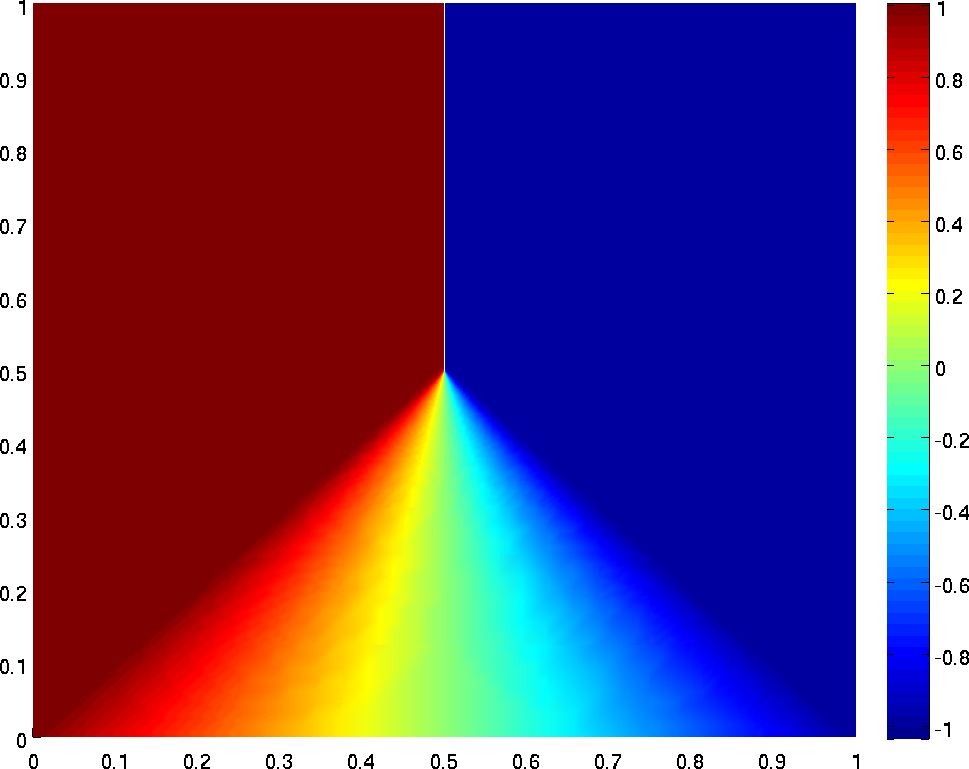
\includegraphics[scale = .35]{figs/burgers1e4.png}
\caption{Shock solution for Burgers' equation, $\epsilon = 1e-4$.}
\end{figure}
\end{column}
\end{columns}
}

\frame{
\frametitle{Compressible Navier-Stokes equations (ideal gas)}
\begin{align*}
\div \vecttwo{\rho u }{\rho v} &= 0\\
\div \left(\vecttwo{\rho u^2+p }{\rho u v} - \boldsymbol \sigma_{1}\right) &=0\\
\div \left(\vecttwo{\rho u v}{\rho v^2+p } - \boldsymbol \sigma_{2}\right) &=0\\
\div \left(\vecttwo{((\rho e)+p)u}{((\rho e)+p)v} - \boldsymbol\sigma \mathbf{u} + \vec{q}\right) &=0\\
\frac{1}{2\mu} \boldsymbol \sigma - \frac{\lambda}{4\mu (\mu + \lambda)} { \rm tr}(\boldsymbol \sigma) \boldsymbol I &= \grad \mathbf{u} - \Reyn \, {\boldsymbol \omega}\\
\frac{1}{\kappa}\vec{q} &= \grad T
\end{align*}
}

\frame{
$\boldsymbol\sigma$ is a Newtonian fluid $\sigma_{ij} = \mu(u_{i,j} + u_{j,i}) + \lambda u_{k,k} \delta_{ij}$.
%We can invert the stress tensor under isotropic and plane strain assumptions to get
\[
\frac{1}{2}\left(\grad  U + \grad ^T  U\right) = \frac{1}{2\mu} \sigma_{ij} - \frac{\lambda}{4\mu (\mu + \lambda)} \sigma_{kk}\delta_{ij}
\]
We also have
\[
\frac{1}{2}\left(\grad  U + \grad ^T  U\right) = \grad  U - \boldsymbol \omega
\]
%where $\boldsymbol \omega$ is the antisymmetric part of the infinitesimal strain tensor:
%\[
%\boldsymbol \omega = \frac{1}{2}\left(\grad  U - \grad ^T  U\right).
%\]
Our final form is
\begin{align*}
\grad  U - \boldsymbol \omega = \frac{1}{2\mu} \boldsymbol \sigma - \frac{\lambda}{4\mu (\mu + \lambda)} { \rm tr}(\boldsymbol \sigma) \boldsymbol I.
\end{align*}
Taking the antisymmetric part implicitly defines $\boldsymbol \omega$ to be the antisymmetric part of $\grad u$. 
}

\frame{
\frametitle{Extrapolation of test norms}
%\begin{columns}
%\begin{column}{.48\textwidth}
Convection-diffusion:
\begin{align*}
\div \left(\beta u - \sigma\right) &= f\\
\frac{1}{\epsilon}\sigma - \grad u &= 0.
\end{align*}
Navier-Stokes:%vectors of test functions  $v=\{v_1,v_2,v_3,v_4\}$, $W = \{\tau_1,\tau_2,\tau_3\}$. Similarly, we group our Eulerian and stress variables into the vector variables $U$ and $\Sigma$.  $R_{\rm Euler}(U,\Sigma)$ and $R_{\rm visc}(U,\Sigma)$ are Eulerian and viscous nonlinear residuals, our formulation for the linearized Navier-Stokes equations can be written as
\begin{align*}
\div \left(A_{\rm Euler}U - A_{\rm visc}\Sigma\right) &= R_{\rm Euler}(U,\Sigma)\\
E_{\rm visc} \Sigma - \grad U &= R_{\rm visc}(U,\Sigma)
\end{align*}
where $R_{\rm Euler}(U,\Sigma)$ and $R_{\rm visc}(U,\Sigma)$ are the Eulerian/viscous residuals.
}

\frame{
Convection-diffusion:
\begin{align*}
\|\left(v,\tau\right)\|_{V,K}^2 =& \min\left\{\frac{\epsilon}{|K|},1\right\}\|v\|^2 + \epsilon \|\grad v\|^2 + \|\beta \cdot \grad v\|^2 \\
&+\| \div \tau\|^2 + \min\left\{\frac{1}{\epsilon},\frac{1}{|K|}\right\}\|\tau\|^2.
\end{align*}

Navier-Stokes: let $V$ and $W$ be vectors of test functions $v_i$ and $\tau_i$.
\begin{align*}
\|\left(V,W\right)\|_{V,K}^2 =& \min\left\{\frac{1}{\Reyn|K|},1\right\}\nor{V}^2 + \frac{1}{\Reyn} \nor{A_{\rm visc}^T\grad V}^2 + \nor{A_{\rm Euler}^T \grad V}^2 \\
& + \nor{\div W}^2 + \min\left\{1,\frac{1}{\Reyn|K|}\right\}\nor{E_{\rm visc}^TW}^2.
\end{align*}
%An advantage of this extrapolation approach is that the incompletely parabolic nature of the Navier-Stokes equation is taken into account; there is no diffusive term present in the mass conservation equation, and the test norm reflects that by requesting only limited regularity of $v_1$.\footnote{The situation is analogous to using the full $H^1(\Oh)$ norm for the pure convection equation --- the optimal test norm $\nor{v}_V = \nor{\beta\cdot \grad v} + \nor{v}$ implies only streamline regularity, whereas taking $\nor{v}_V = \nor{\grad v} + \nor{v}$ implies stronger regularity on the test space $V$ than the graph norm. Consequently, convergence is suboptimal for DPG applied to the convection problem under the $H^1(\Oh)$ test norm.}
%\end{column}
%\end{columns}
}
\frame{
\frametitle{Carter plate and Boundary conditions}

\begin{figure}[!h]
\centering
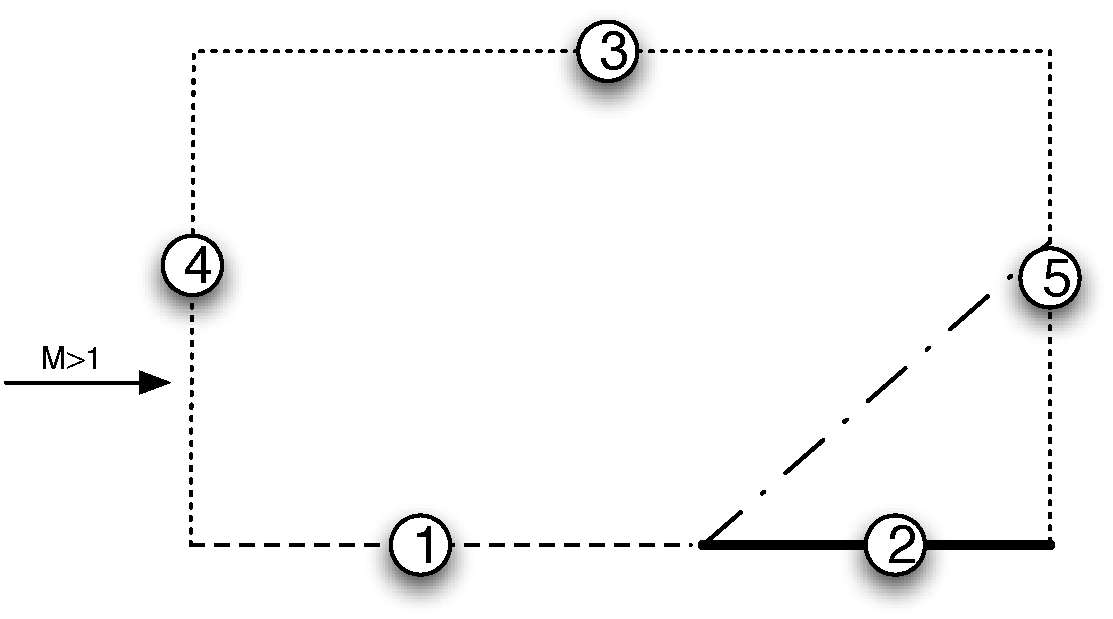
\includegraphics[scale=.35]{figs/flat_plate_BCs.pdf}
\caption{Carter flat plate problem.}
\end{figure}
\begin{itemize}
\item{} Inflow and stress boundary conditions, momentum flux boundary conditions. 
\item{} No outflow condition set.
\end{itemize}
}

\frame{
\frametitle{Refinement level 0}
\begin{figure}
\subfigure[$u_1$]{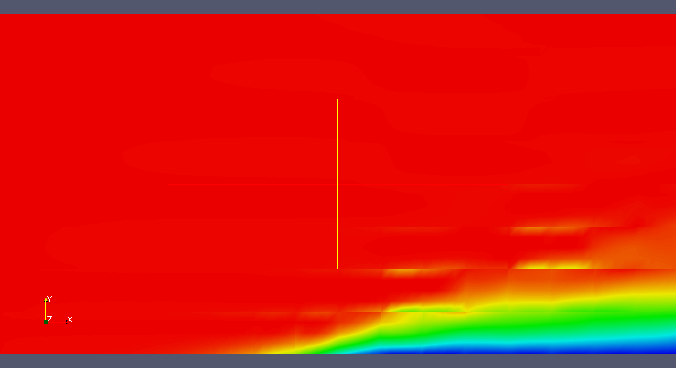
\includegraphics[scale = .23]{figs/Re1000p2/u10.png}}
\subfigure[$T$]{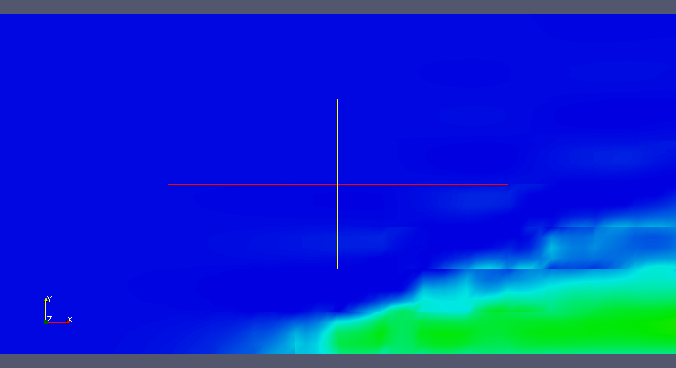
\includegraphics[scale = .23]{figs/Re1000p2/T0.png}}
\subfigure{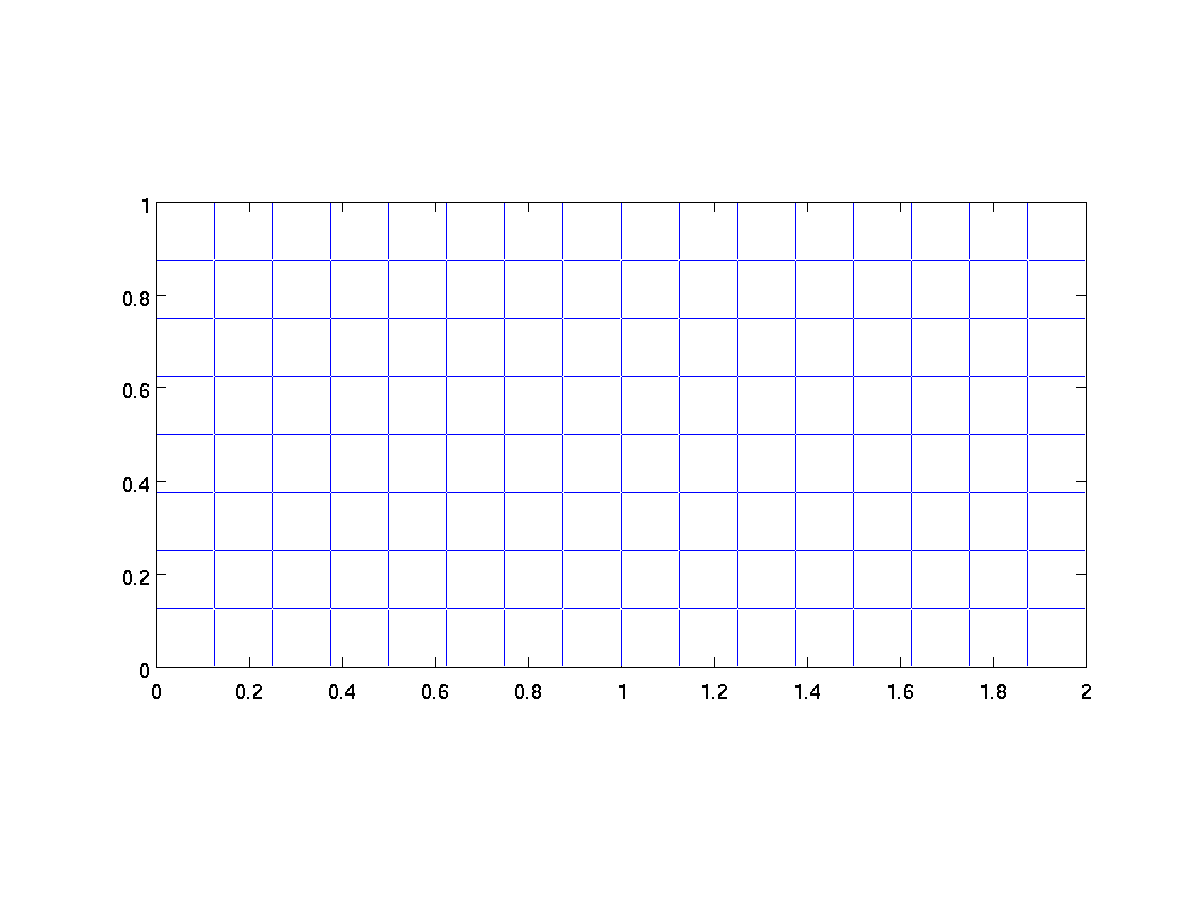
\includegraphics[scale = .35]{figs/Re1000p2/mesh0.png}}
\end{figure}
}
\setcounter{subfigure}{0}

\frame{
\frametitle{Refinement level 1}
\begin{figure}
\subfigure[$u_1$]{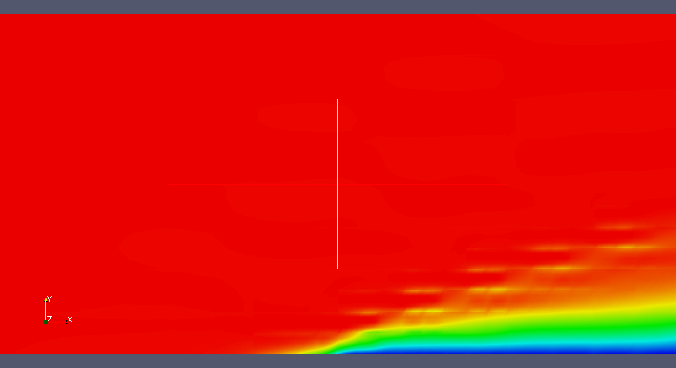
\includegraphics[scale = .23]{figs/Re1000p2/u11.png}}
\subfigure[$T$]{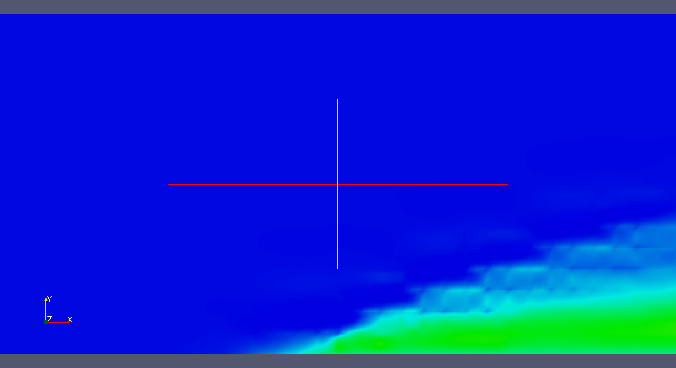
\includegraphics[scale = .23]{figs/Re1000p2/T1.png}}
\subfigure{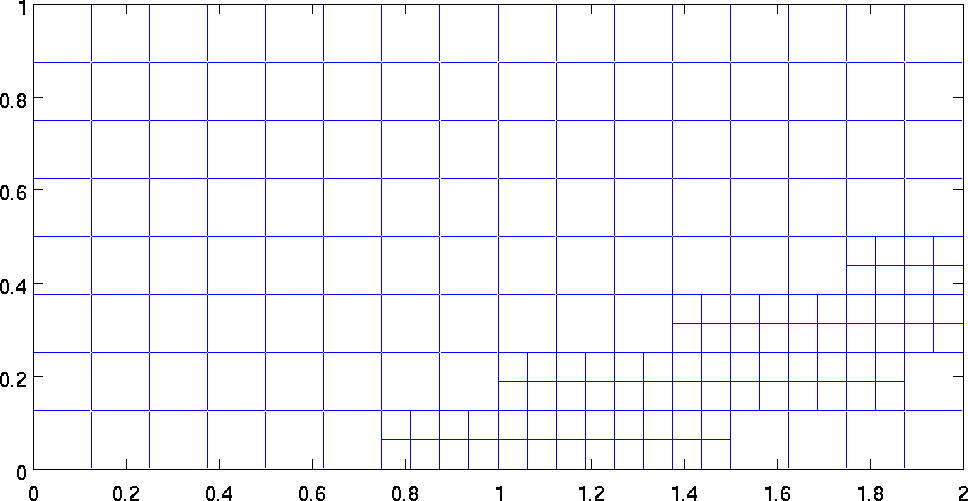
\includegraphics[scale = .35]{figs/Re1000p2/mesh1.png}}
\end{figure}
}
\setcounter{subfigure}{0}

\frame{
\frametitle{Refinement level 2}
\begin{figure}
\subfigure[$u_1$]{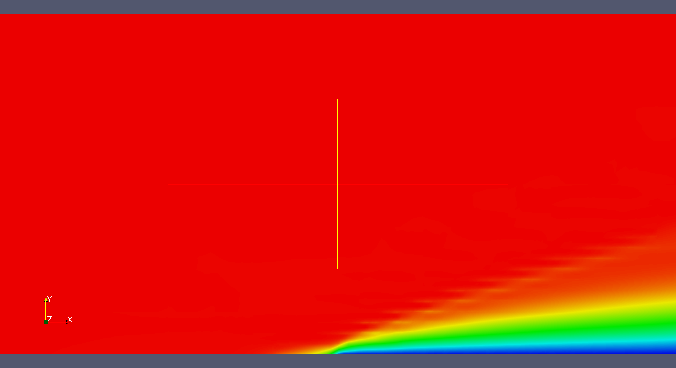
\includegraphics[scale = .23]{figs/Re1000p2/u12.png}}
\subfigure[$T$]{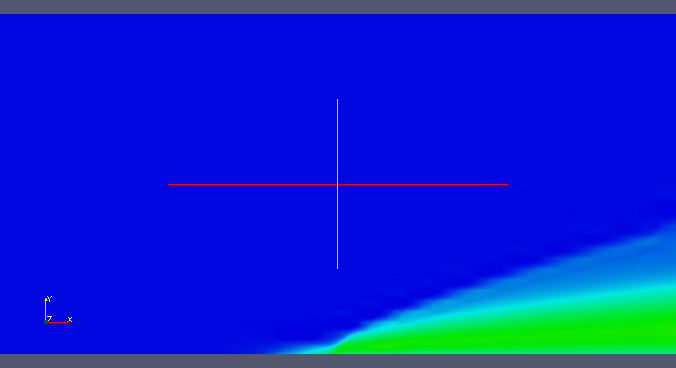
\includegraphics[scale = .23]{figs/Re1000p2/T2.png}}
\subfigure{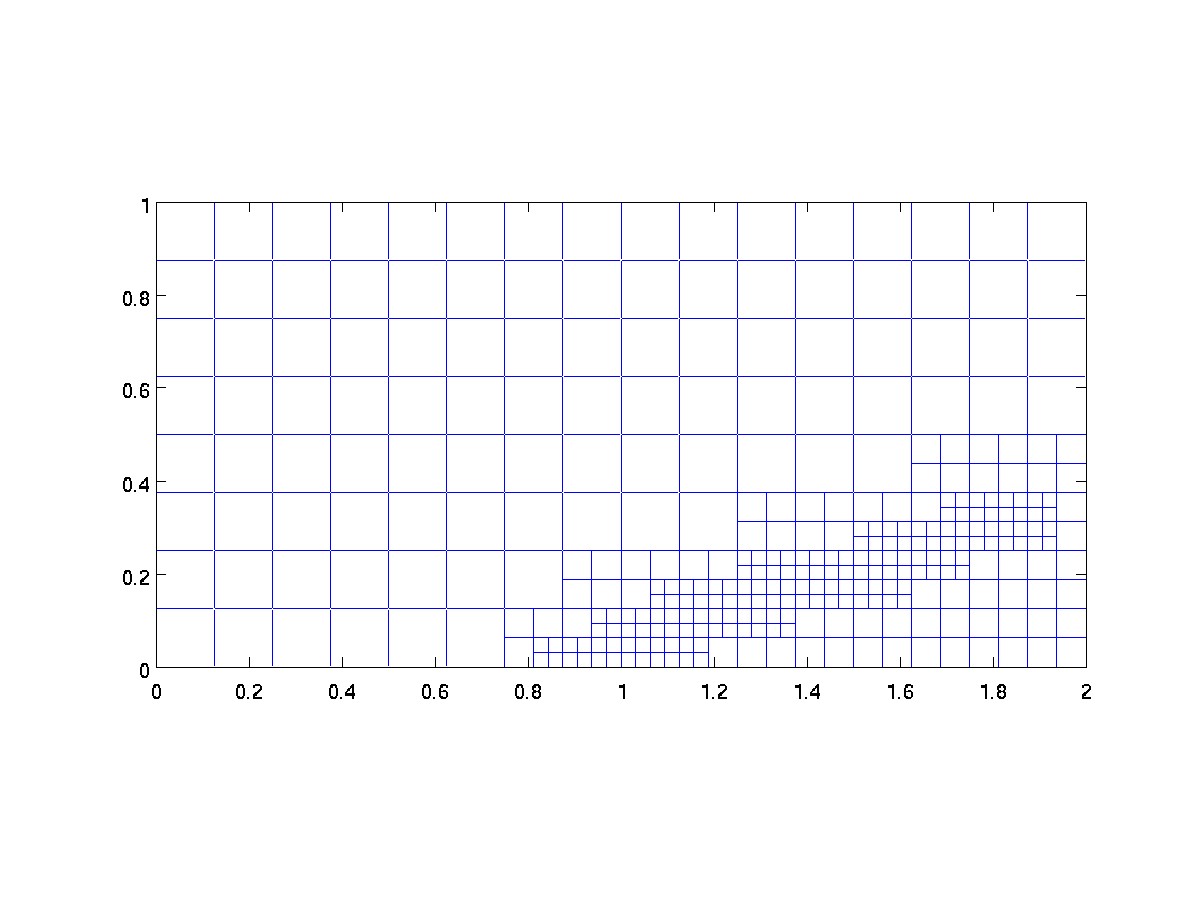
\includegraphics[scale = .35]{figs/Re1000p2/mesh2.png}}
\end{figure}
}
\setcounter{subfigure}{0}

\frame{
\frametitle{Refinement level 3}
\begin{figure}
\subfigure[$u_1$]{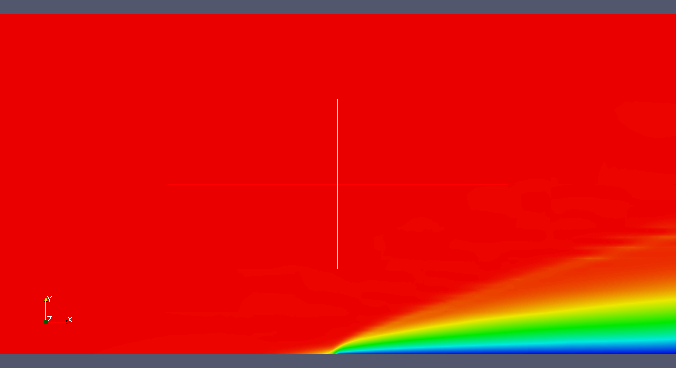
\includegraphics[scale = .23]{figs/Re1000p2/u13.png}}
\subfigure[$T$]{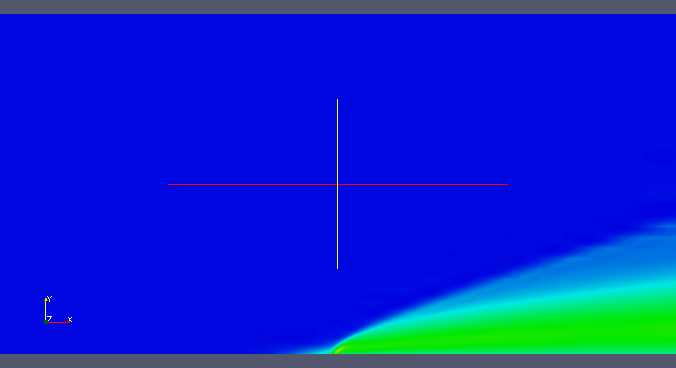
\includegraphics[scale = .23]{figs/Re1000p2/T3.png}}
\subfigure{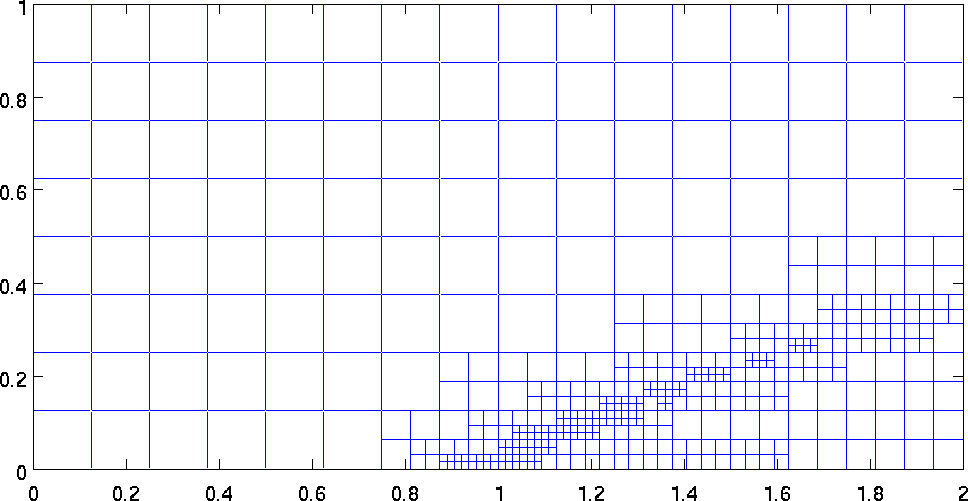
\includegraphics[scale = .35]{figs/Re1000p2/mesh3.png}}
\end{figure}
}
\setcounter{subfigure}{0}

\frame{
\frametitle{Refinement level 4}
\begin{figure}
\subfigure[$u_1$]{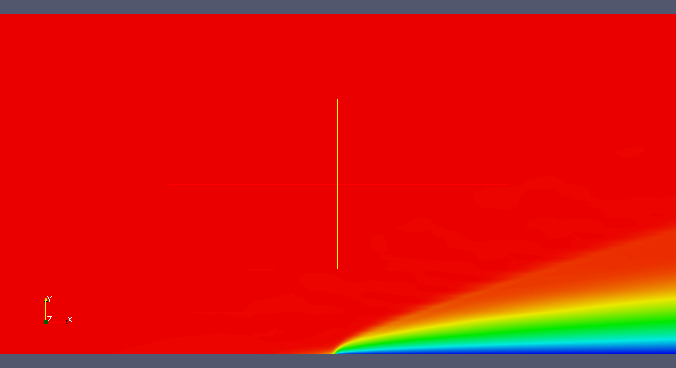
\includegraphics[scale = .23]{figs/Re1000p2/u14.png}}
\subfigure[$T$]{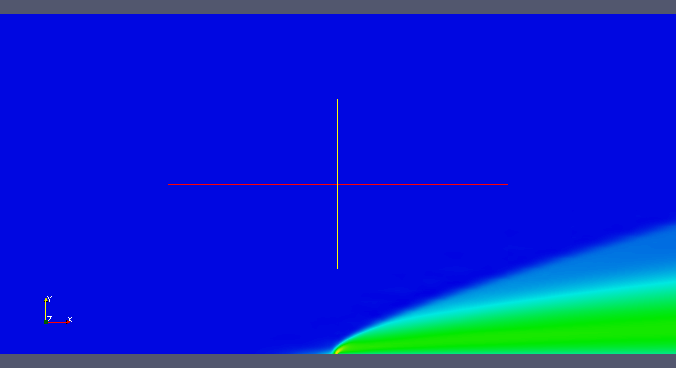
\includegraphics[scale = .23]{figs/Re1000p2/T4.png}}
\subfigure{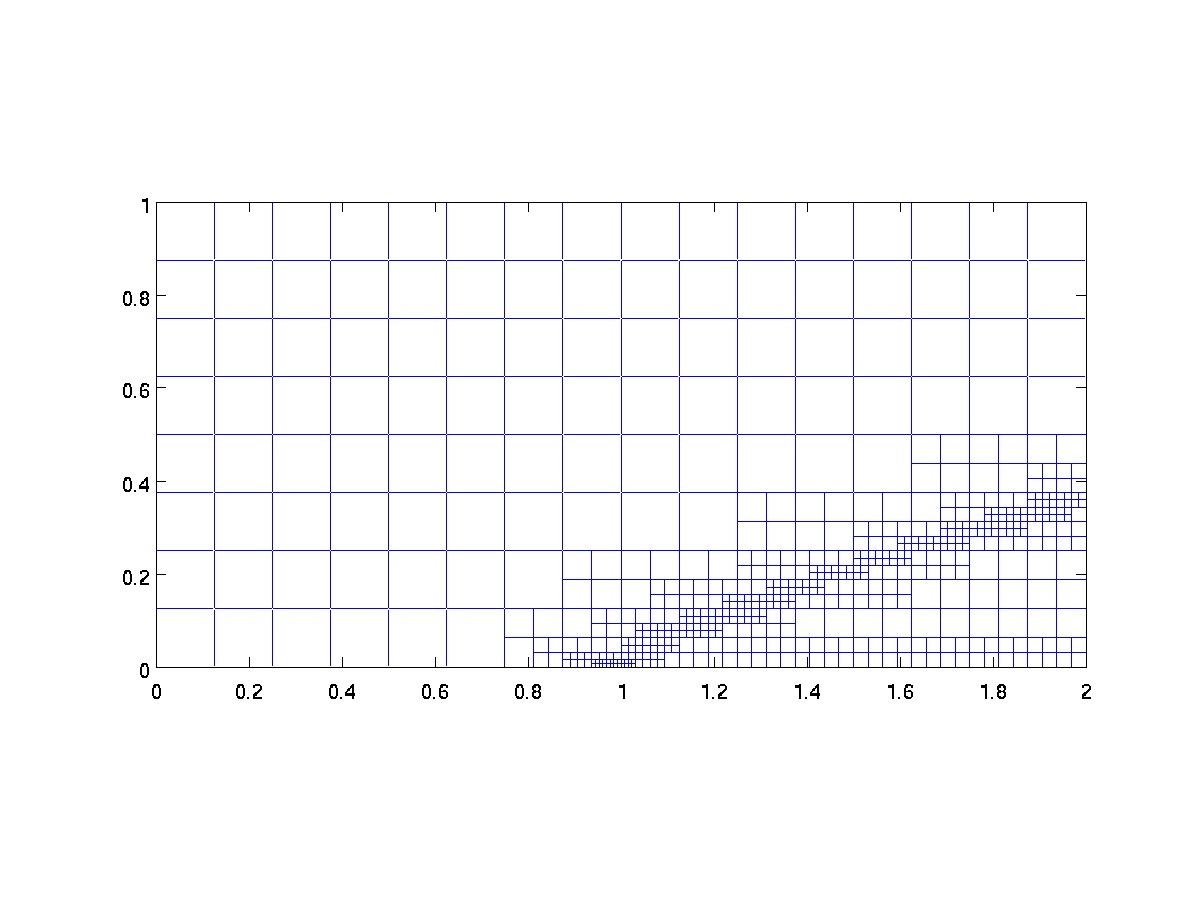
\includegraphics[scale = .35]{figs/Re1000p2/mesh4.png}}
\end{figure}
}
\setcounter{subfigure}{0}

\frame{
\frametitle{Refinement level 5}
\begin{figure}
\subfigure[$u_1$]{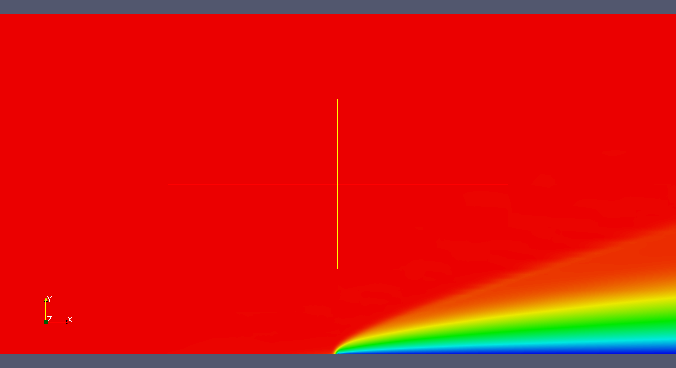
\includegraphics[scale = .23]{figs/Re1000p2/u15.png}}
\subfigure[$T$]{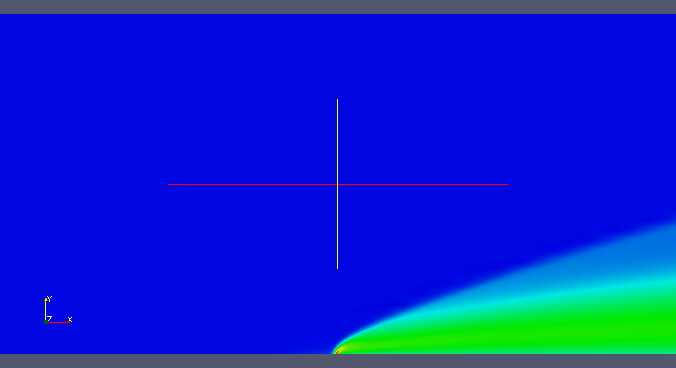
\includegraphics[scale = .23]{figs/Re1000p2/T5.png}}
\subfigure{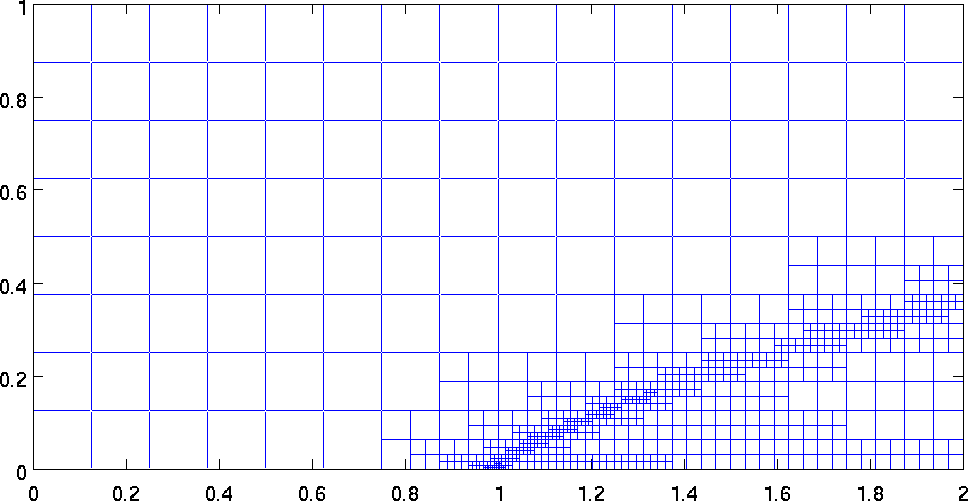
\includegraphics[scale = .35]{figs/Re1000p2/mesh5.png}}
\end{figure}
}
\setcounter{subfigure}{0}

\frame{
\frametitle{Refinement level 6}
\begin{figure}
\subfigure[$u_1$]{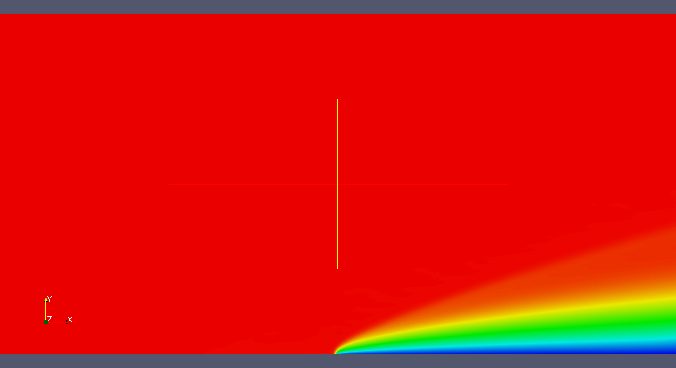
\includegraphics[scale = .23]{figs/Re1000p2/u16.png}}
\subfigure[$T$]{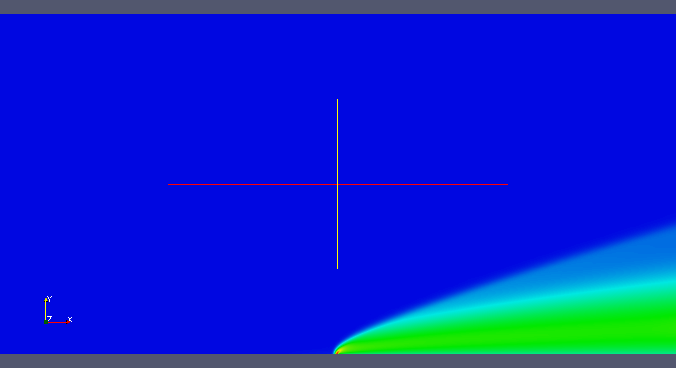
\includegraphics[scale = .23]{figs/Re1000p2/T6.png}}
\subfigure{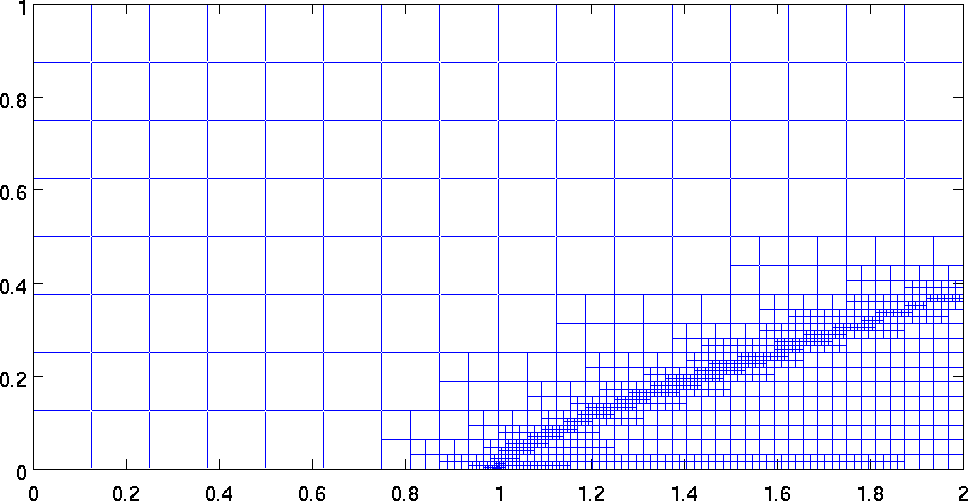
\includegraphics[scale = .35]{figs/Re1000p2/mesh6.png}}
\end{figure}
}
\setcounter{subfigure}{0}

\frame{
\frametitle{Zoomed solutions at the plate edge}
\begin{figure}
\subfigure[$\rho$]{\includegraphics[scale = .12]{figs/Re1000p2/rhoUnscaledzoom.png}}
\subfigure[$u_1$]{\includegraphics[scale = .12]{figs/Re1000p2/u1zoom.png}}
\subfigure[$u_2$]{\includegraphics[scale = .12]{figs/Re1000p2/u2zoom.png}}
\subfigure[$T$]{\includegraphics[scale = .12]{figs/Re1000p2/Tzoom.png}}
\subfigure[$q_n$]{\includegraphics[scale = .23]{figs/Re1000p2/heatflux.png}}
\end{figure}
}

\section{Proposed work}
\subsection{Area A}
\frame{
\frametitle{Proposed work: Area A}
\begin{itemize}
\item{\textbf{Completed: Prove robustness of DPG method for the scalar convection-diffusion problem.}}

We have introduced a test norm under which the DPG method robustly bounds the $L^2$ error in the field variables $u$ and the scaled stress $\sigma$. Numerical results confirm the theoretical bounds given. 

\item{\textbf{Proposed: Attempt analysis of the linearized Navier-Stokes system.}}

We hope to analyze the linearized Navier-Stokes equations to determine an optimal extrapolation of the test norm for the scalar convection-diffusion problem to systems. 

\end{itemize}
}

\subsection{Area B}

\frame{
\frametitle{Future work: Area B}
\begin{itemize}
\item{\textbf{Completed: Collaborative work with Nathan Roberts on the higher order parallel adaptive DPG code Camellia.}}

Numerical experiments use the higher-order adaptive codebase Camellia, built upon the Trilinos library by Nathan Roberts. %The framework for arbitrary-irregularity anisotropic refinements in both $h$ and $p$ is in place, and the code is partially parallelized.

\item{\textbf{Proposed: Anisotropic refinements and $hp$-schemes.}}

The error representation function drives refinement effectively, and we hope to generalize its use to anisotropic adaptive schemes. 
\begin{figure}
\subfigure{\includegraphics[scale = .18]{figs/anisotropy/b5.png}}
\subfigure{\includegraphics[scale = .186]{figs/anisotropy/v6.png}}
\end{figure}
\end{itemize}
}

\frame{
\textbf{Proposed: Distributed iterative static condensation.}
\[
Ku = \arr{A}{B}{B^T}{D}\vecttwo{u_{\rm flux}}{u_{\rm field}} = \vecttwo{f}{g} = l
\]
where $D$ has a block-diagonal structure. The system can be reduced to yield the condensed system
\[
\left(A-B D^{-1} B^T\right)u_{\rm flux} = f - B D^{-1} g
\]
where $D^{-1}$ can be inverted block-wise. For FE stiffness matrices under the Laplace equation, the Schur complement has reduced condition number of $O(h^{-1})$ as opposed to $O(h^{-2})$. 
}

\frame{  
\textbf{Proposed: a Nonlinear Hessian-based DPG method.}
Given a nonlinear variational problem $b(u,v) = l(v)$, linear in $v$ but not in $u$, beginning with the \textit{nonlinear} dual residual 
\[
J(u_h) = \frac{1}{2}\|B(u_h)-l\|_{V'}^2 \coloneqq\frac{1}{2} \sup_{v\in V\setminus\{0\}} \frac{| b(u_h,v)-l(v)|^2}{\nor{v}_V^2}.
\]
produces a Hessian-based DPG method, which solves
\[
b_u(\Delta u,v) + b''(\Delta u, \delta u, v_{R(u)}) = l(v) - b(u,v) = r(u,v),
\]
and aims to minimize the nonlinear dual residual instead of the linearized problem residual. 
}

\subsection{Area C}
\frame{
\frametitle{Proposed work: Area C}
\begin{itemize}
\item{\textbf{Completed: convection-dominated diffusion, Burgers, and a model problem for Navier-Stokes.}} 
\item{\textbf{Proposed: Range of Reynolds/Mach numbers, ramp problem, Gaussian bump.}}
\item{\textbf{Proposed: regularized Euler.}}
%\textcolor{red}{Graphics?}
\end{itemize}
}
\end{document}
